%% -----------------------------------------------------------------------------

\chapter{Evaluation}\label{ch:evaluation}
\glsresetall % Resets all acronyms to not used
\glsunset{IEEE} \glsunset{MAC}

In this chapter, the proposed technique for detecting sender \gls{MAC} addresses during collisions is evaluated using several simulations as well as experiments on \gls{WARP} \glspl{SDR}.

Possible questions and problems include the fact that with higher \glspl{MCS}, there might be not enough samples to correlate the rather short six byte \gls{MAC} address. Another interesting issue is the accuracy of the algorithm with increasing amounts of noise and fading.


%% -----------------------------------------------------------------------------

\section{Frequency-Domain Correlation}\label{sec:freqd-correlation}

During the implementation of the \gls{MAC} address detection technique, I tried using cross-correlation in the frequency-domain. This means that instead of calculating the similarity between samples, complex symbols are correlated without mapping them into the time-domain. With this approach, the Fourier transform must be applied to the received signal.

It turns out to be very difficult, if not impossible, to detect senders in case of a collision with frequency-domain correlation. The reason for that is phase shift due to path delays. When a signal is received with an offset in the time-domain, the constellation is changed in the frequency-domain. This can be shown using the Fourier transform equation:

$$ F(f) = \int_{-\infty}^{\infty} s(t) \cdot e^{-2 \pi i f t} dt $$\vspace{0cm}

Here, $ i $ is the imaginary unit, $ F(f) $ is the Fourier transform at frequency $ f $, and $ s(t) $ is the time-domain signal depending on $ t $. A time offset can now be expressed as $ t + \Delta $. Standard power laws then show that this offset introduces a constant multiplication factor on $ F(f) $, depending on $ \Delta $.

$$ F(f) = \int_{-\infty}^{\infty} s(t + \Delta) \cdot e^{-2 \pi i f \cdot (t + \Delta)} dt = \int_{-\infty}^{\infty} s(t + \Delta) \cdot e^{-2 \pi i f t} \cdot e^{-2 \pi i f \Delta} dt = $$
$$ = e^{-2 \pi i f \Delta} \cdot \int_{-\infty}^{\infty} s(t + \Delta) \cdot e^{-2 \pi i f t} dt $$\vspace{0cm}

Since both $ s(t) $ and $ F(f) $ are complex functions, this multiplication is a rotation, or phase shift, in the complex constellation plane. Furthermore, the rotation is different for diverse frequencies $ f $.

Due to the way \gls{OFDM} works, a received signal will contain a variety of frequencies within the channel bandwidth. All those frequencies experience a different phase shift. This leads to a received constellation similar to that shown in figure \ref{fig:freqd-corr}. To create this figure, I applied a Rayleigh channel \cite{sklar1997} to a simulated collision signal, introducing a delay of a few nanoseconds. The signals are modulated with \gls{BPSK}, so ideally the only constellation points should be $ 1 $ and $ -1 $. However, due to the above described rotation, the constellation is basically a circle.

\begin{figure}[ht]
	\centering
	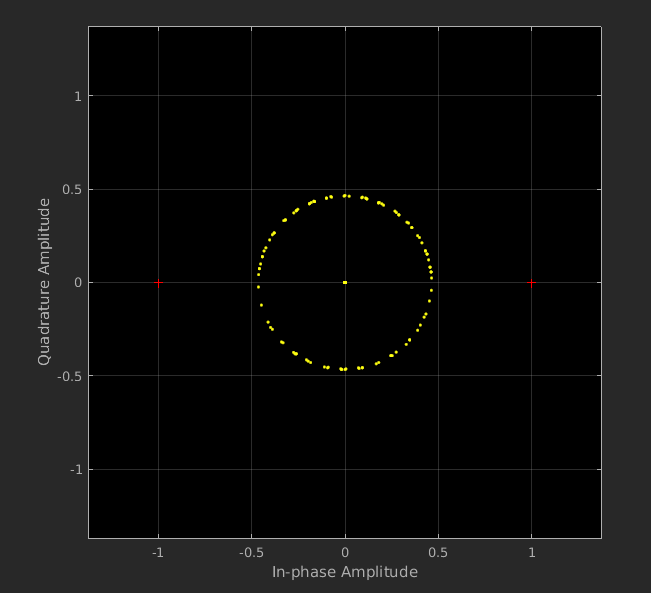
\includegraphics[width=8cm]{gfx/images/freqd-correlation}
	\caption{Cross Correlation of Frequency-Domain Symbols after Channel}
	\label{fig:freqd-corr}
\end{figure}

This kind of path effects is not at all unusual in a IEEE 802.11 transmission. Under normal circumstances, the known preamble is used to calculate the inverted channel matrix of the path effects \cite{perahia2013}, as mentioned in section \ref{sec:multipath}.\\

When receiving a collision, there is however not only one preamble. Instead, the preambles of two different frames, that experienced different path effects, are added together. Since the preambles themselves are designed to have a low off-peak autocorrelation \cite{ieee2012}, it is not easily possible to separate the two channel effects from each other.

This is caused by the receiver, which would normally correlate the received training field with a local copy, and estimate the phase shift present in the complex cross-correlation. For this reason, I can not reverse the phase shift introduced on the \gls{OFDM} symbols containing the \gls{MAC} address. It is therefore not possible to detect which sender transmitted the frame.

As expected, experiments with cross-correlation in the frequency-domain without channel equalization were unsuccessful. I therefore disregarded this approach.


%% -----------------------------------------------------------------------------

\section{Time-Domain Correlation}

The experiments I did using time-domain cross-correlation are divided into two groups. First, I used Matlab to simulate different field variations and channel effects. Second, I used WARP boards to try the approach in a real-world scenario. The results of these experiments are summarized in the following sections \ref{sec:ex-mcs} to \ref{sec:ex-warp}.

When correlating time-domain samples, I used pre-generated reference samples and calculated the correlation only for the subset of samples that contains the \gls{MAC} address. Section \ref{sec:mac-periods} describes which period of the signal this is.\\

Reference signals are modulated until just after the \gls{IFFT} and adding of cyclic prefix. For the simulations, I used a sampling rate of 20 MHz, which is the default output of the Matlab WLAN System Toolbox. The WARP boards use a sampling frequency of 40 MHz however, so for these experiments I used interpolation to double the rate.

All experiments used real-world \gls{MAC} addresses, as described in section \ref{sec:real-world-macs}.


%% -----------------------------------------------------------------------------

\section{Real-World MAC Addresses}\label{sec:real-world-macs}

\gls{MAC} addresses are six byte long numbers, where the first three bytes are a vendor prefix, identifying the company that built the network interface. The remaining three bytes are a unique identifier for the specific hardware.

After initial tries with some artificial \gls{MAC} addresses in the form of \texttt{AB:CD:EF:12:34:56}, I switched to using a sample set of real-world \gls{MAC} addresses. This allowed for a closer simulation of an actual use-case for sender detection.\\

I collected 64 \gls{MAC} addresses from devices that were connected to the wireless university eduroam network. The gathering was done in the afternoon on a weekday. I used airodump from the \texttt{aircrack-ng} software suite\footnote{https://www.aircrack-ng.org/} to dump all \gls{MAC} addresses on the network into a file. The actual command looked like this:

\begin{lstlisting}[captionpos=b,caption={Capture Real-World MAC Addresses},label=lst:airodump]
airmon-ng start wlp0s20u1
airodump-ng --essid eduroam -a -o csv -w mac-addresses-eduroam.csv wlp0s20u1mon
\end{lstlisting}

It is important to have the wireless network interface set to promiscuous mode. This mode instructs the driver to hand all received frames to the kernel. Otherwise, only frames that are going to or coming from the local station are gathered, while the rest is filtered. This means that only the router's and the station's own \gls{MAC} address would be cached.

In a possible real-time usage scenario of the sender detection algorithm, it would also be important to use promiscuous mode in order to collect all \gls{MAC} addresses. These are the addresses for which reference signals need to be modulated and cached.


%% -----------------------------------------------------------------------------

\section{Modulation and Coding Schemes}\label{sec:ex-mcs}

Intuitively, the overall sender detection accuracy should decrease for higher \glspl{MCS}. First, with a higher \gls{MCS} there are more payload bits encoded in every \gls{OFDM} symbol, as seen in table \ref{tbl:mcs}. This means that when applying cross-correlation, the \gls{OFDM} symbol contains random data from the \gls{MAC} header before and after the sender \gls{MAC} address. Due to the nature of \gls{OFDM}, it is not possible to limit correlation to only a fraction of the symbol in the time-domain.

Second, a higher \gls{MCS} means that payload data gets mapped to complex points in the constellation plane that are less distinct from each other. Therefore, different data can be more similar under cross-correlation, making it harder to detect senders in the time-domain.\\

To evaluate the detection algorithm's performance, I measured the correctness of detected \gls{MAC} addresses for each of the eight available \glspl{MCS}. For every \gls{MCS}, 1000 runs were performed with a new randomly chosen sender pair on each run. The results are stacked sums of runs where a completely correct pair of senders were guessed, times where only one of the senders was correct, and the number of failures, in the sense of both addresses being incorrect.

\begin{figure}[H]
	\centering
	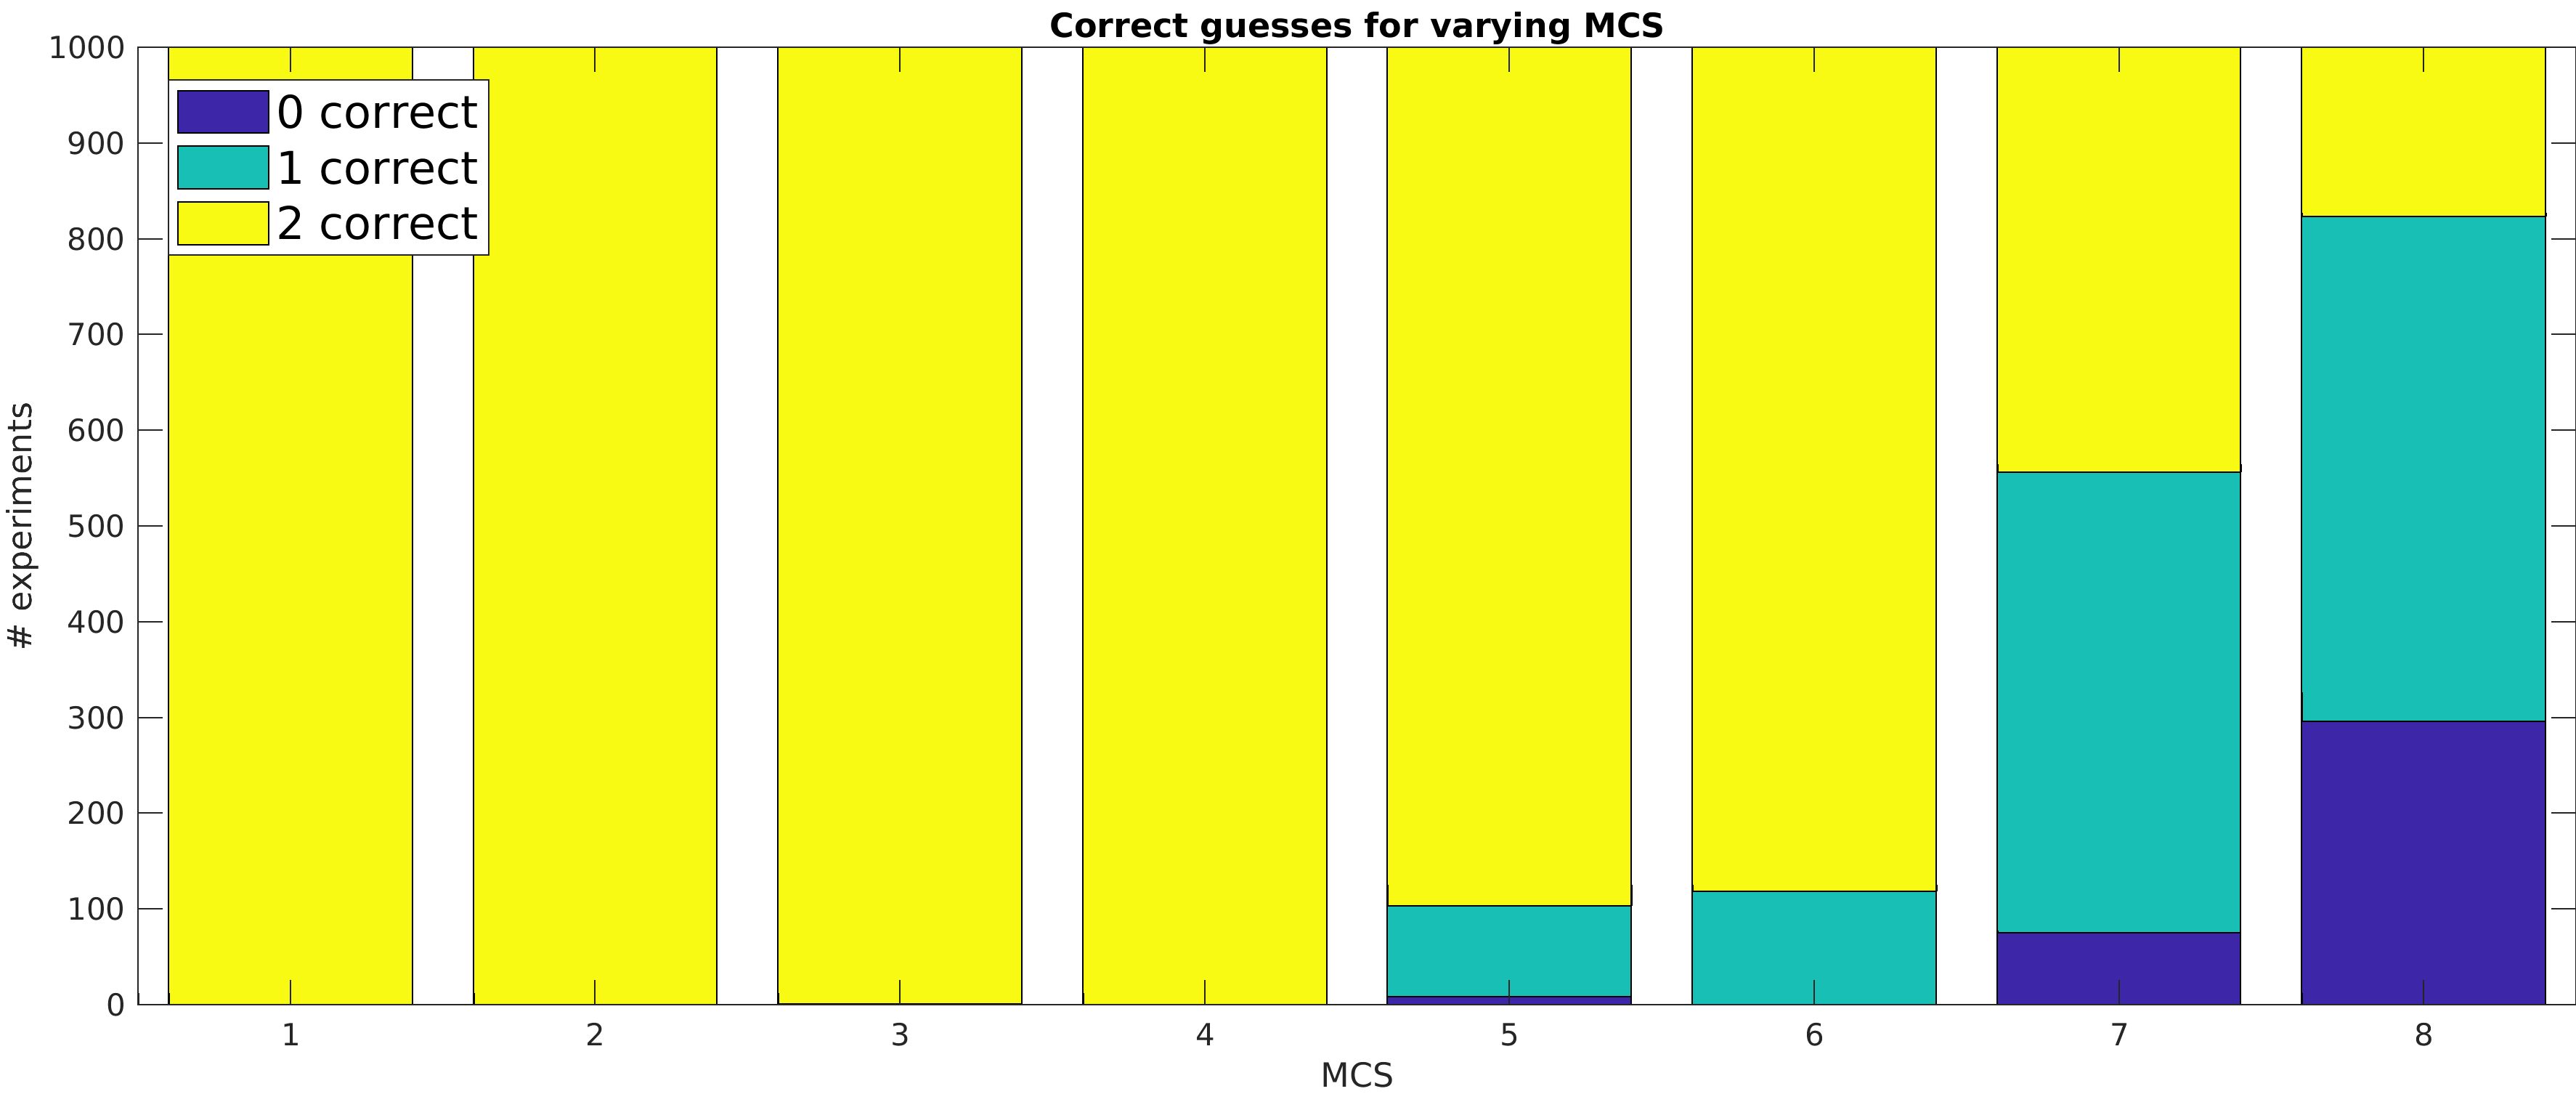
\includegraphics[height=4.5cm]{gfx/plots/mcs}
	\caption{Results: Varying MCS for 1000 Runs}
	\label{fig:vary_mcs}
\end{figure}

Figure \ref{fig:vary_mcs} shows the resulting plot. Different \glspl{MCS} are spread out on the x axis. The stacked bars show the number of experiments for each result category as described above. As expected, the detection accuracy decreases for higher \glspl{MCS}. It is worth mentioning that for low \glspl{MCS}, the performance is very good, better than I expected. Furthermore, it seems to decrease exponentially, but to justify this more data would be needed.


%% -----------------------------------------------------------------------------

\section{Scrambler Initialization}\label{sec:ex-scrambler}

As described in section \ref{sec:mac-and-phy}, the \gls{MAC} layer payload data is scrambled before any modulation on the physical layer is applied. The scrambling uses a seven bit state register, where 0 is no valid state. Therefore, 127 unique scrambler initialization values are possible.

If the scrambler initialization is important for the sender detection technique, specifically if the modulated reference signals must use the same initialization as the received frames, the number of possible values linearly scales the algorithm's complexity. That is, for every cached \gls{MAC} address, \gls{MCS}, et cetera all scrambler initializations must be modulated and correlated. It is therefore very interesting to know whether this is the case, or whether the scrambler does not affect detection quality.\\

Figure \ref{fig:vary_scrambler} shows the detection performance for different scrambler initializations over 1000 runs. The data is presented the same way as in the previous section. The stacked bar plots denote the number of runs with zero, one, and two corrects guesses. For all experiments, the \gls{MCS} 0 was used. While the simulated received frame was modulated with scrambler initialization 1, correlation was calculated against 127 reference signals with different scrambler values.

\begin{figure}[H]
	\centering
	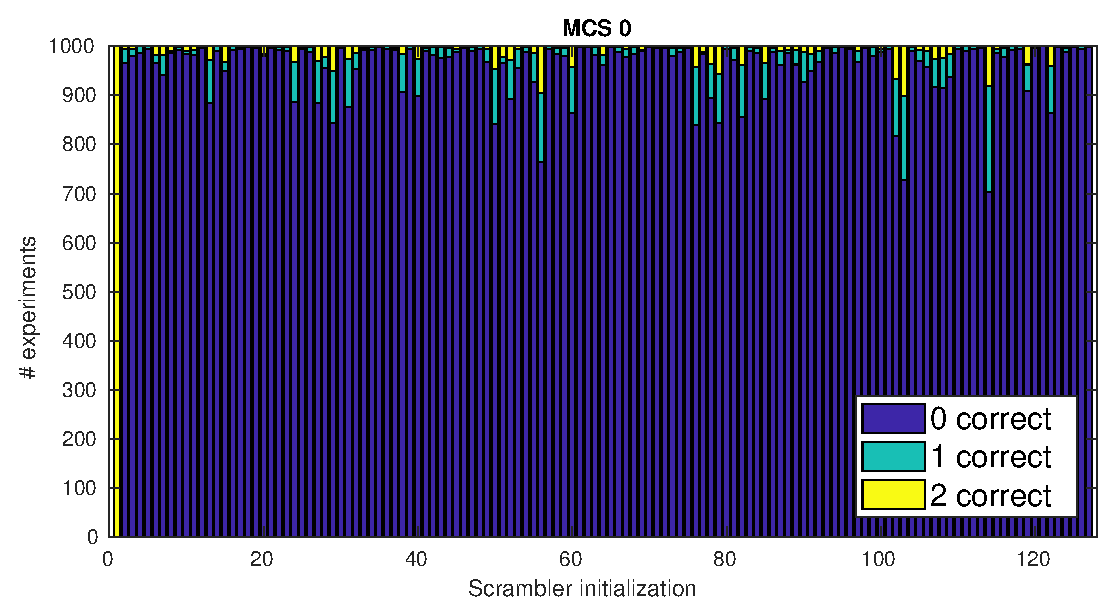
\includegraphics[height=4.5cm]{gfx/plots/scrambler}
	\caption[Results: Varying Scrambler Initialization for 1000 Runs]{Results: Varying Scrambler Initialization for 1000 Runs at MCS 0}
	\label{fig:vary_scrambler}
\end{figure}

The results show that the scrambler initialization is very important for detection quality. While the performance is very good for the correct initialization value 1, for all other values the accuracy is low. However, related research mentions that some network interfaces seem to not choose the scrambler initialization at random \cite{noubir2016}, contradictory to the IEEE 802.11 standard. These devices use a static initialization for every frame, or increment the value after every transmission. This could be exploited by limiting the reference signals to the ones that are expected in the current network. This avoids time being spent on correlations that are unpromising. Since the \gls{MAC} addresses of stations in the network are cached, the interface types and vendors are known. This could lead to some interesting future work.

Another important task is to identify when the correct scrambler initialization for a given frame is used and hence a sender guess is meaningful. Since the initialization values of collided frames are unknown, every possible value has to be tried and correlated. The sender guess is based on highest probability, meaning there is a guess regardless of whether a correlation is using the right scrambling sequence. Therefore, receivers need to detect which sender guess is the most promising one. This should be possible by using a threshold for cross-correlation peaks and could be explored in following work.


%% -----------------------------------------------------------------------------

\section{Preceding Data Variations}\label{sec:ex-destination}

Similar to the scrambler initialization, the \gls{MAC} header field preceding the sender \gls{MAC} address could also influence detection quality. This is due to the convolutional encoder as described in section \ref{sec:mac-and-phy}. Since it uses a state register to calculate the encoding, the output bits are dependent on previous input. Therefore, it could be necessary to address all possible values of preceding data in order to generate suitable reference signals for all MAC addresses. The field before the sender \gls{MAC} address in a data frame is the destination \gls{MAC} address. In the following experiment, I measured to which extent the value of the destination address affects the accuracy of my detection technique. The scrambler initialization was 1 for all runs of this experiment.\\

Figure \ref{fig:vary_dest} shows the results in the same way as for the previous figures. Since the convolutional encoder uses a seven bit state, only the last seven bits of the destination \gls{MAC} address matter. After these last seven bits, the register is synchronized to the same state, regardless of the preceding first 41 bits of the address. This makes up for a total of 128 different values that are evaluated with 1000 runs each. Unlike the scrambler initialization, results are presented for \gls{MCS} 1 here. At \gls{MCS} 0, there were no recognition errors at all, yielding a less interesting plot.

\begin{figure}[H]
	\centering
	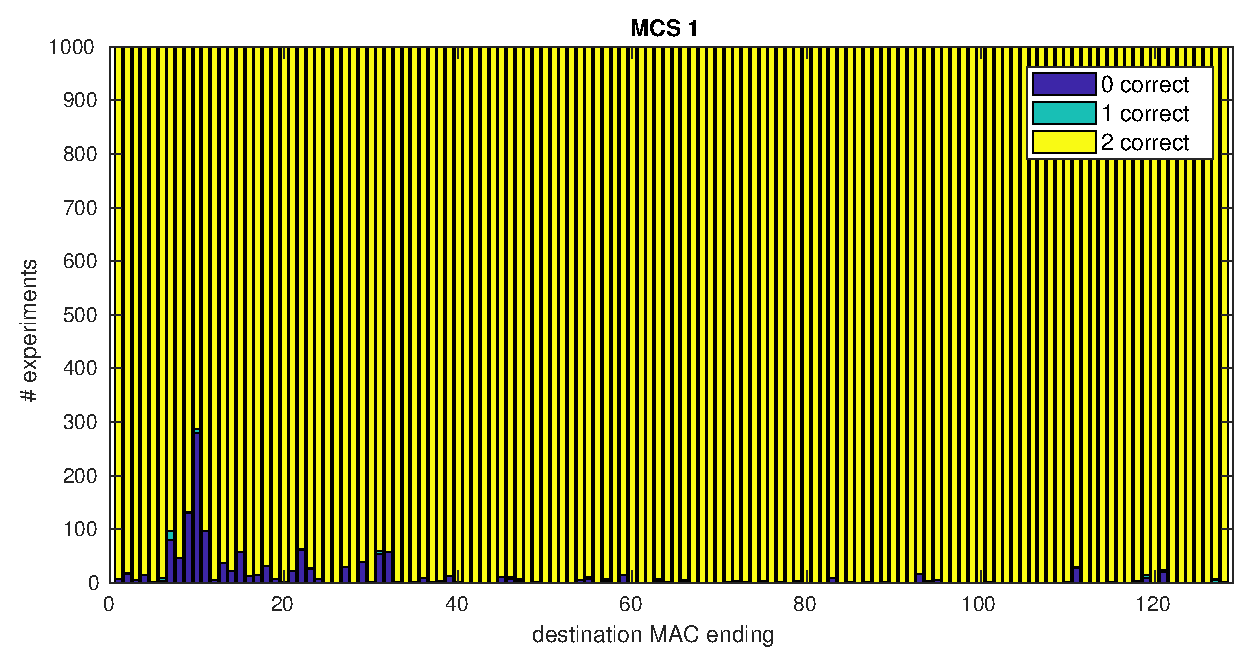
\includegraphics[height=4.5cm]{gfx/plots/destination}
	\caption[Results: Varying Destination \gls{MAC} Address for 1000 Runs]{Results: Varying Destination \gls{MAC} Address for 1000 Runs at MCS 1}
	\label{fig:vary_dest}
\end{figure}

It turns out that unlike the scrambler initialization, preceding payload data does not really have a measurable effect. Detection quality is comparable regardless of the trailing bits of the \gls{MAC} address. I discuss possible reasons for this in section \ref{sec:detection-quality}. An important implication of this result is that it is not necessary to check all 128 possible encoder states for every collision in real-time, which would be another linear scaling factor for the computational complexity of the algorithm.


%% -----------------------------------------------------------------------------

\section{Channel Models}

So far, all experiments were done in simulations with an ideal channel, meaning there were no path effects such as multi-path fading or attenuation. I evaluate performance under various channel models in this section.\\

Using Matlab, there are different models available that could be applied. First, I begin with applying \gls{AWGN} with different \glspl{SNR}. While \gls{AWGN} is not specifically modeled for IEEE 802.11 networks and will therefore not replicate channel conditions precisely, it is a good starting point. The \gls{SNR} is measured in decibel, and swept from $ -20 $ to $ 60 dB $.

The results of the experiments are shown in figure \ref{fig:vary_awgn}. For each \gls{SNR} and every \gls{MCS}, 1000 experiment runs were performed.\\

Second, the Communications System Toolbox comes with \texttt{stdchan}, which supports the \texttt{802.11a} and \texttt{802.11g} channel types. These are suited quite well for this scenario. The channel models require some parameters, including the sampling frequency, Doppler spread, and \gls{RMS} delay spread $ t_{\text{RMS}} $. The delay spread was varied from 100 ns to 500 ns in steps of 50 ns. The usage of the stdchan filter is illustrated by listing \ref{lst:stdchan}:

\begin{lstlisting}[captionpos=b,caption={Matlab stdchan Channel Model},label=lst:stdchan]
trms = ...; % 30, 40, etc.
fs = 20e6; % Hz Sampling Frequency
fd = 10; % Hz Doppler spread
chan = stdchan(1/fs, fd, '802.11g', trms);
rx = filter(chan, tx);
\end{lstlisting}

The results of this experiment are shown in figure \ref{fig:vary_trms}. For each $ t_{\text{RMS}} $ value, 1000 runs were performed. The process was repeated for all eight \glspl{MCS}.\\

Third, the WLAN System Toolbox comes with a number of specifically drafted IEEE 802.11 channel models. These are designed according to the IEEE 802.11 standard models described in the specification \cite{ieee2012}. There are six models (A to F), of which I used the following three:

\begin{itemize}
	\item \textit{Model B}: typical large open space and office environments, no line-of-sight, 100 ns \gls{RMS} delay spread
	\item \textit{Model D}: large open space (indoor and outdoor), line-of-sight conditions, 140 ns \gls{RMS} delay spread
	\item \textit{Model E}: typical large open space (indoor and outdoor), no line-of-sight, 250 ns \gls{RMS} delay spread
\end{itemize}

I used the \texttt{wlanTGnChannel} class. Technically, this channel is designed to be used with IEEE 802.11 n high-throughput networks. However, the class supports configuration of \gls{MIMO} streams. I set those to one antenna for transmission and reception, respectively. This should provide appropriate conditions for \gls{SISO} 802.11 a/g networks.

The channel is used with Matlab code similar to listing \ref{lst:tgn}. As for the \texttt{stdchan} invocation, the sampling rate is passed to the function. I use path-loss and shadowing for fading, and configure \gls{SISO}.

\begin{lstlisting}[captionpos=b,caption={Matlab wlanTGnChannel Simulation},label=lst:tgn]
model = ...; % 'Model-B', 'Model-D', etc.
tgnchan = wlanTGnChannel( ...
        'SampleRate', 20e6, ... % Hz
        'LargeScaleFadingEffect', 'Pathloss and shadowing', ...
        'NumTransmitAntennas', 1, 'NumReceiveAntennas', 1, ... % SISO
        'DelayProfile', model);
rx = tgnchan(tx);
\end{lstlisting}

The results of the experiments are shown in figure \ref{fig:vary_tgn}. For each of the three channel models and every \gls{MCS}, 1000 runs were performed.\\

I conclude that \glspl{MCS} 0 to 2 allow to detect senders quite well under channel effects. For these, \gls{AWGN} caused almost no measurable impact. Even \texttt{stdchan}, which seems to have the biggest effect on detection quality, showed good results. For higher \glspl{MCS} however, accuracy quickly decreased significantly. The combination of high \gls{RMS} delay spread under the Standard Channel model with \gls{MCS} starting from 3 yielded almost no entirely correct guesses.

\begin{figure}[p]
	\centering
	\begin{tabular}{cc}
		\subfloat[MCS 0]{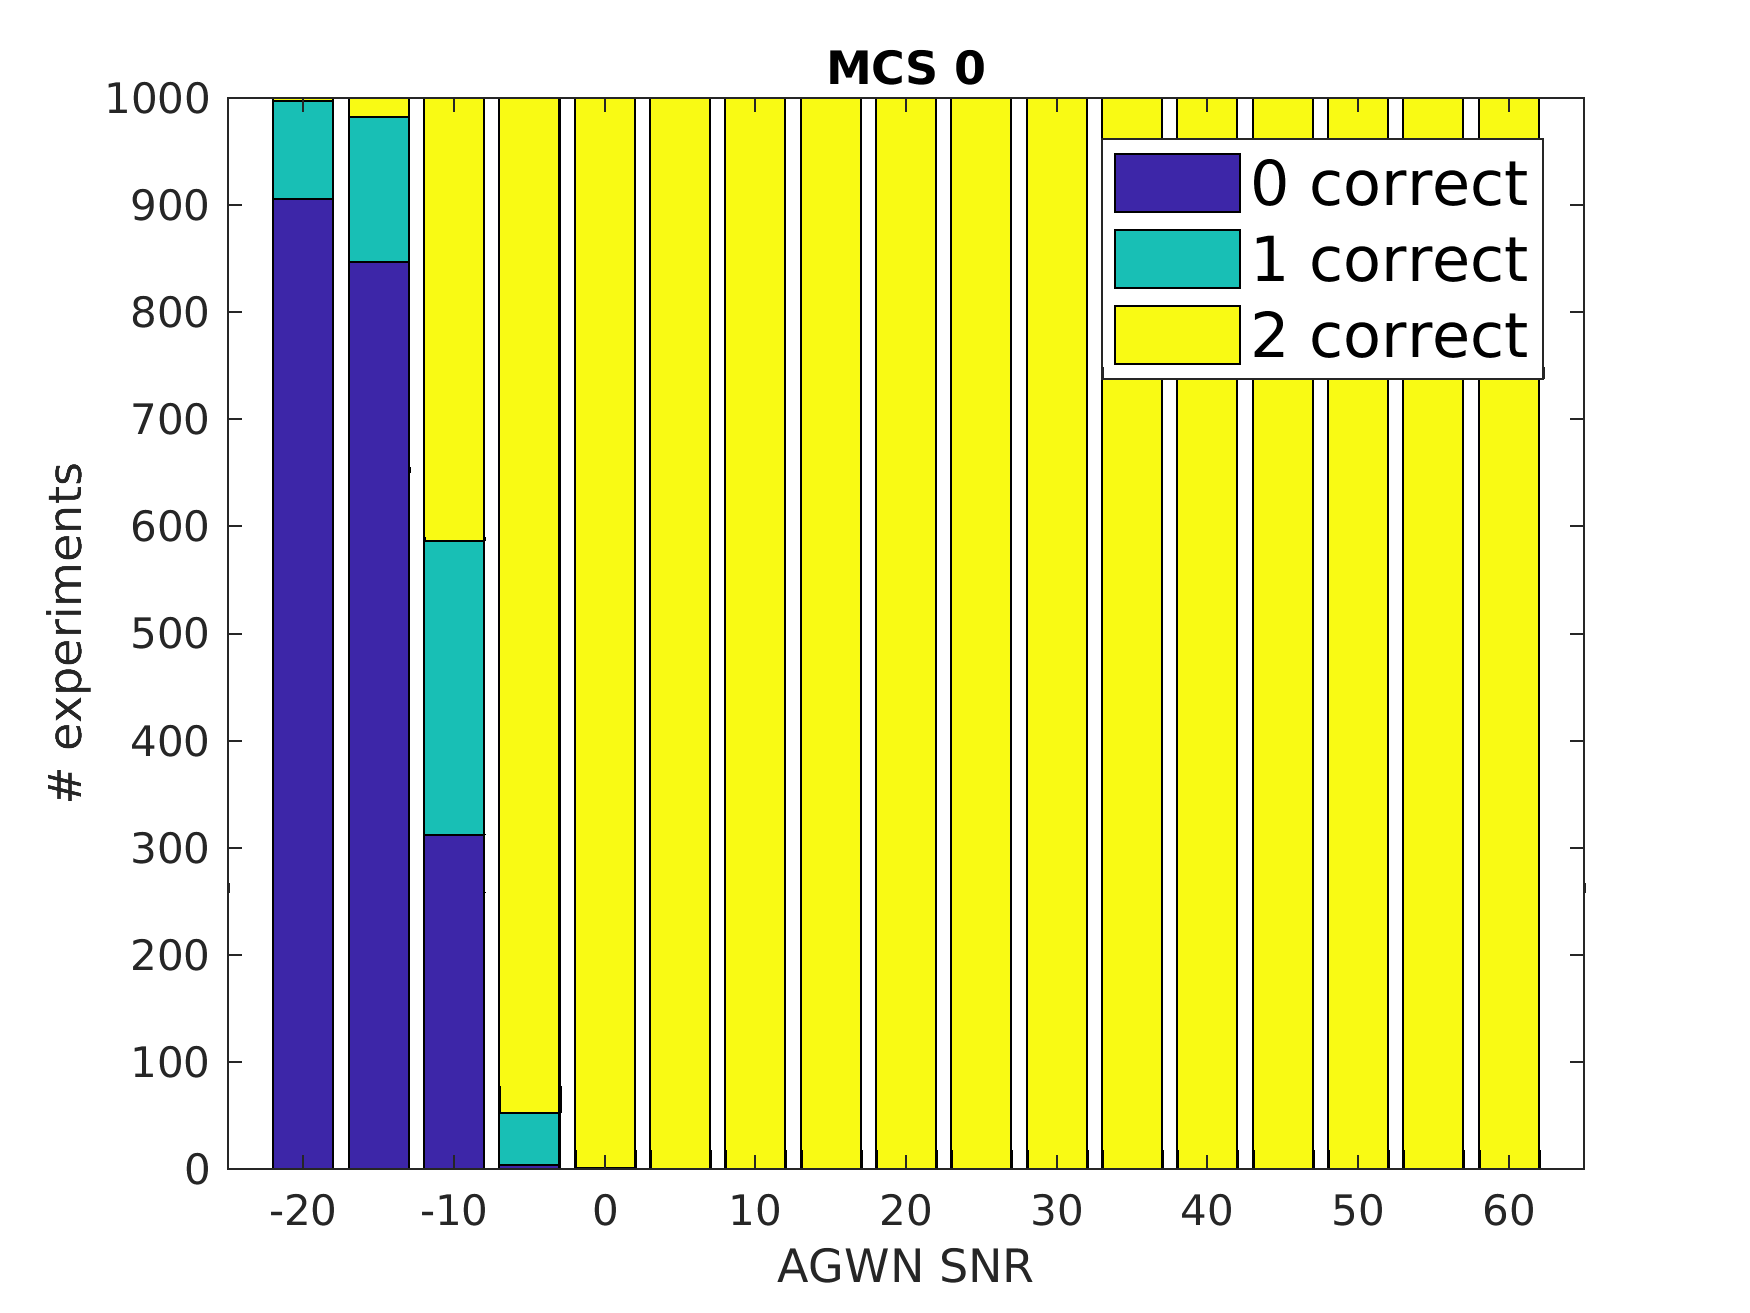
\includegraphics[width=0.42\textwidth]{gfx/plots/awgn-mcs0}} &
		\subfloat[MCS 1]{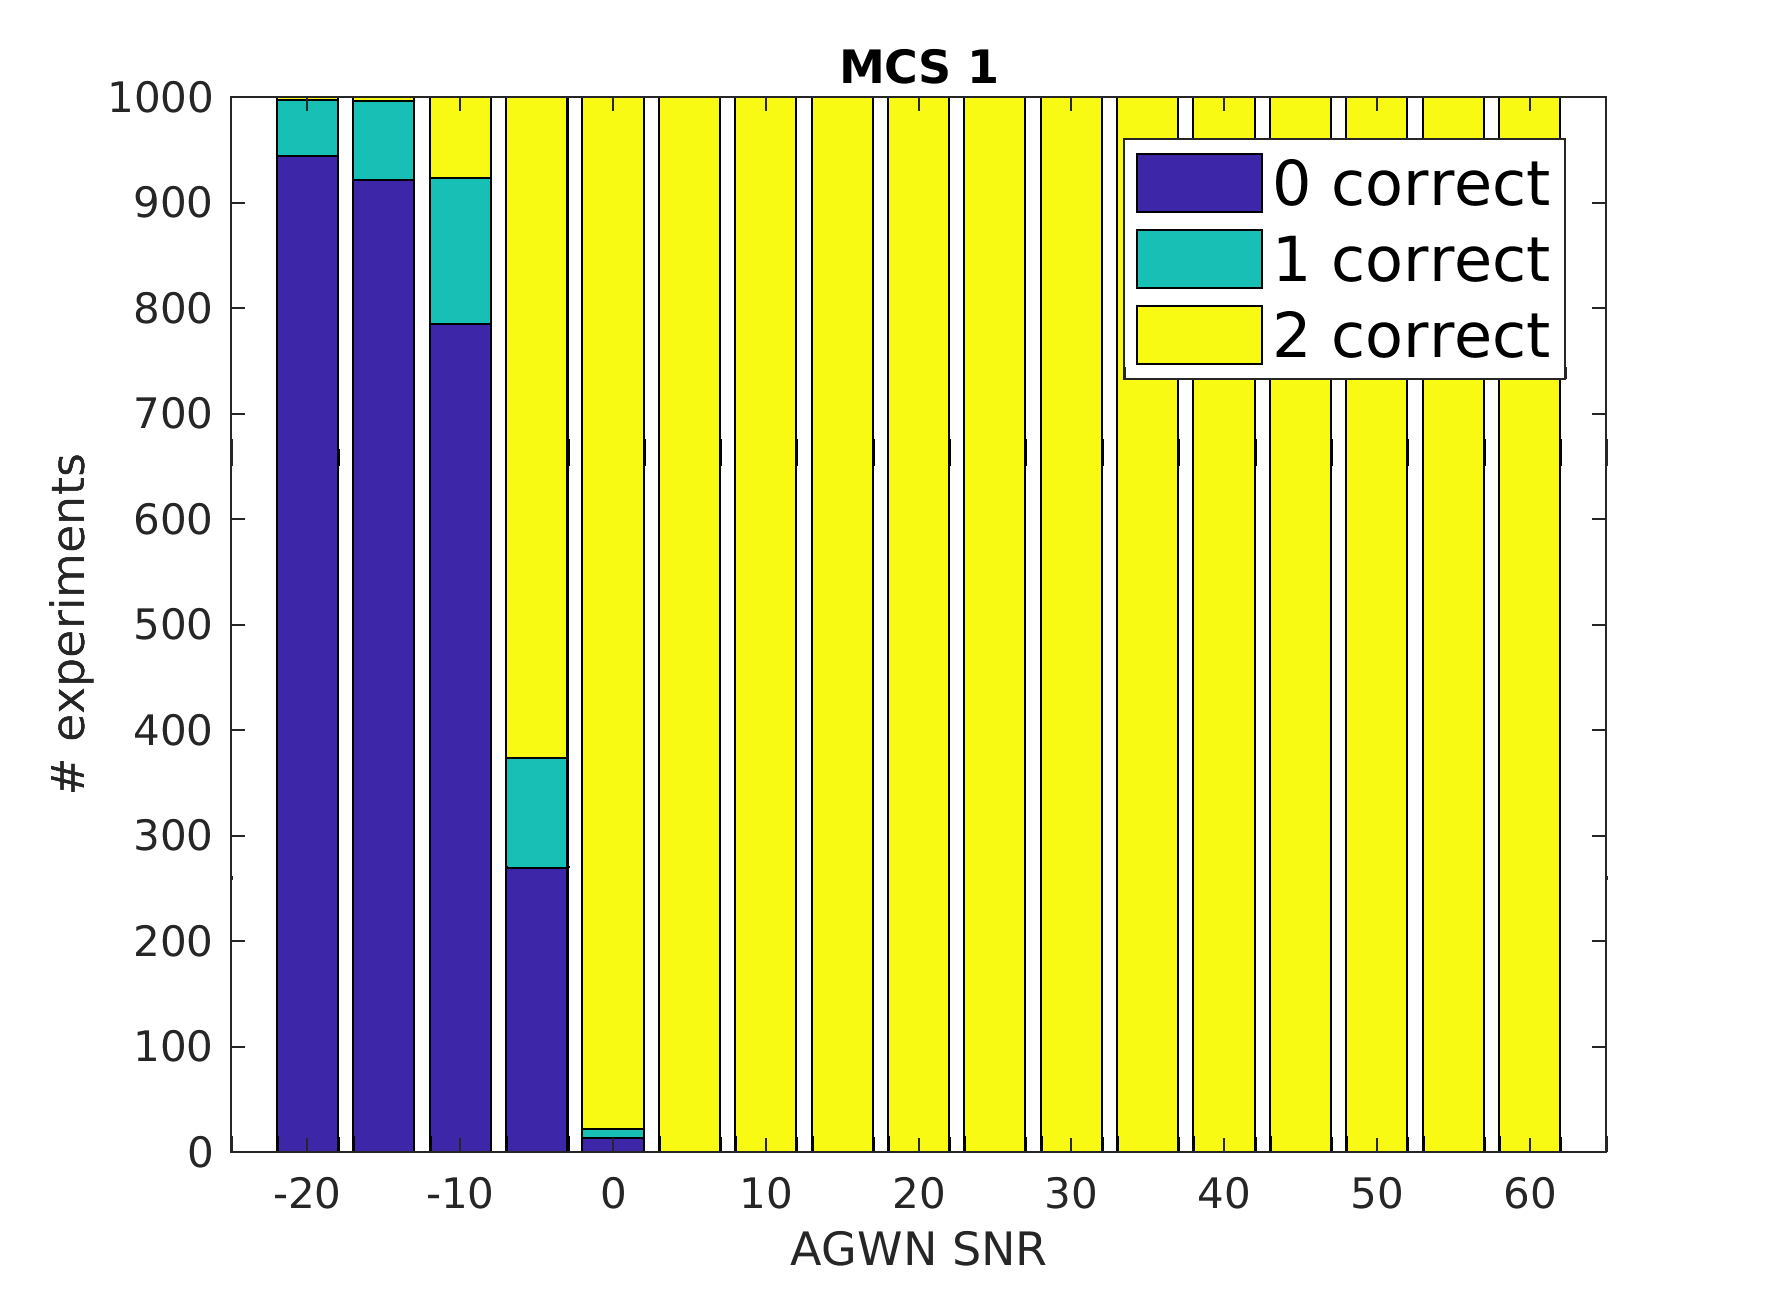
\includegraphics[width=0.42\textwidth]{gfx/plots/awgn-mcs1}} \\
		\subfloat[MCS 2]{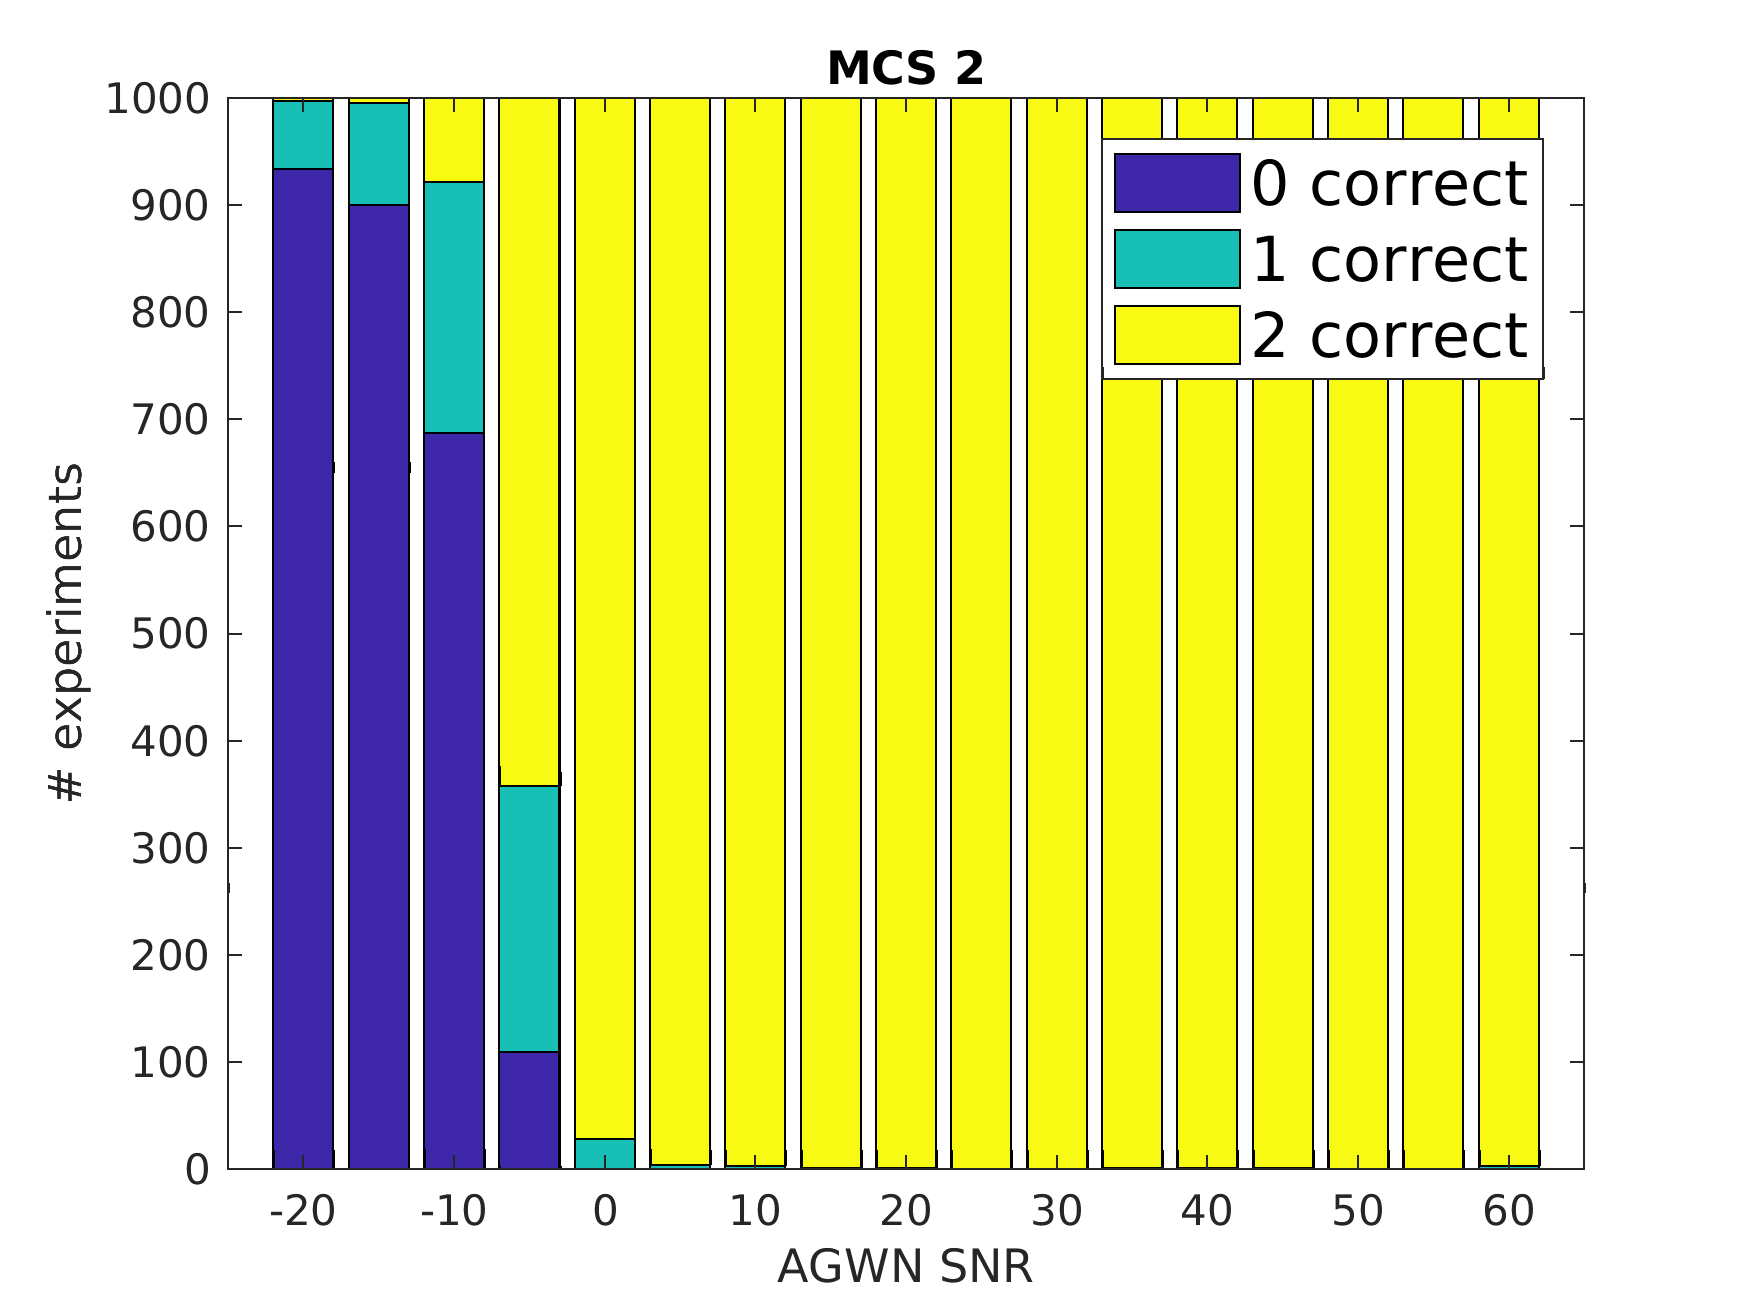
\includegraphics[width=0.42\textwidth]{gfx/plots/awgn-mcs2}} &
		\subfloat[MCS 3]{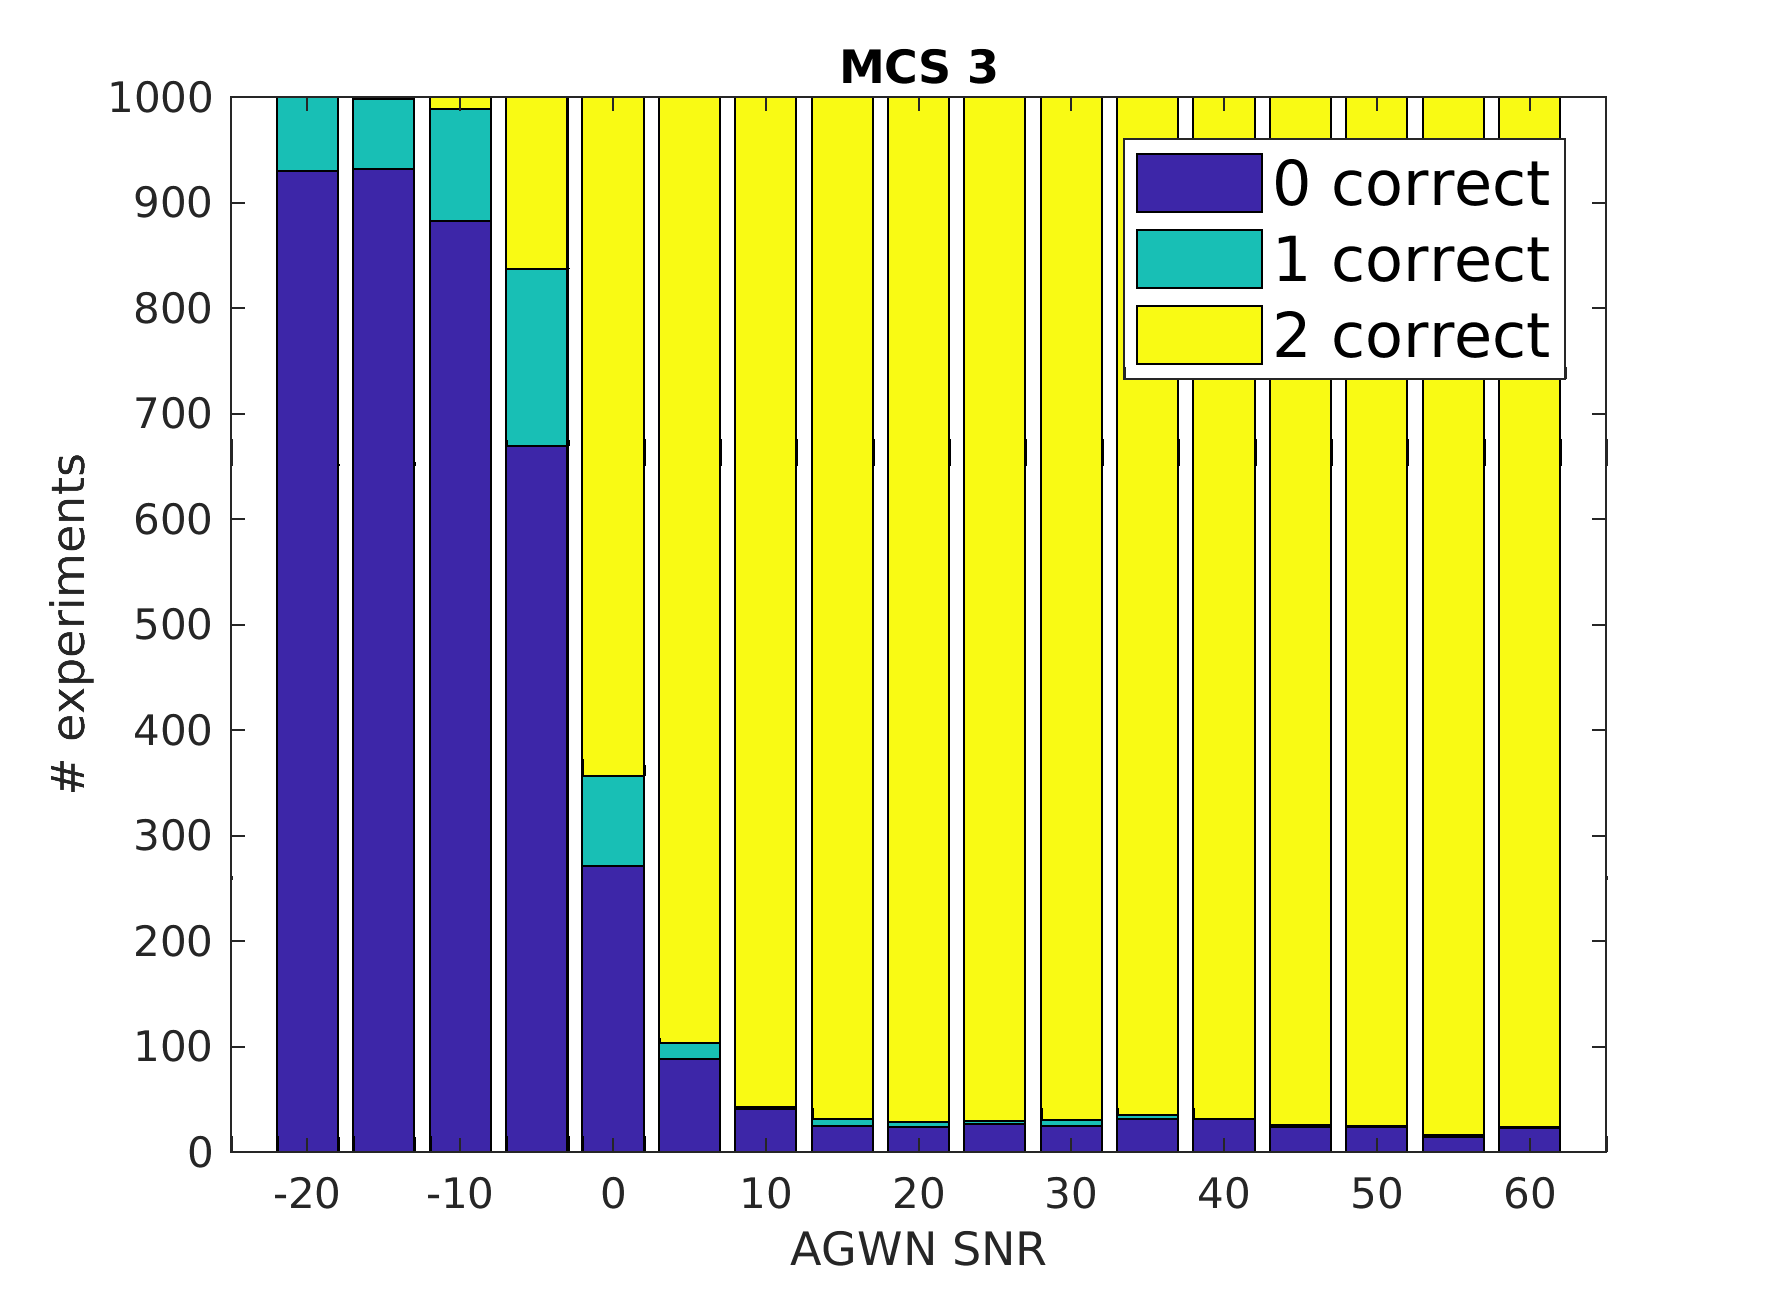
\includegraphics[width=0.42\textwidth]{gfx/plots/awgn-mcs3}} \\
		\subfloat[MCS 4]{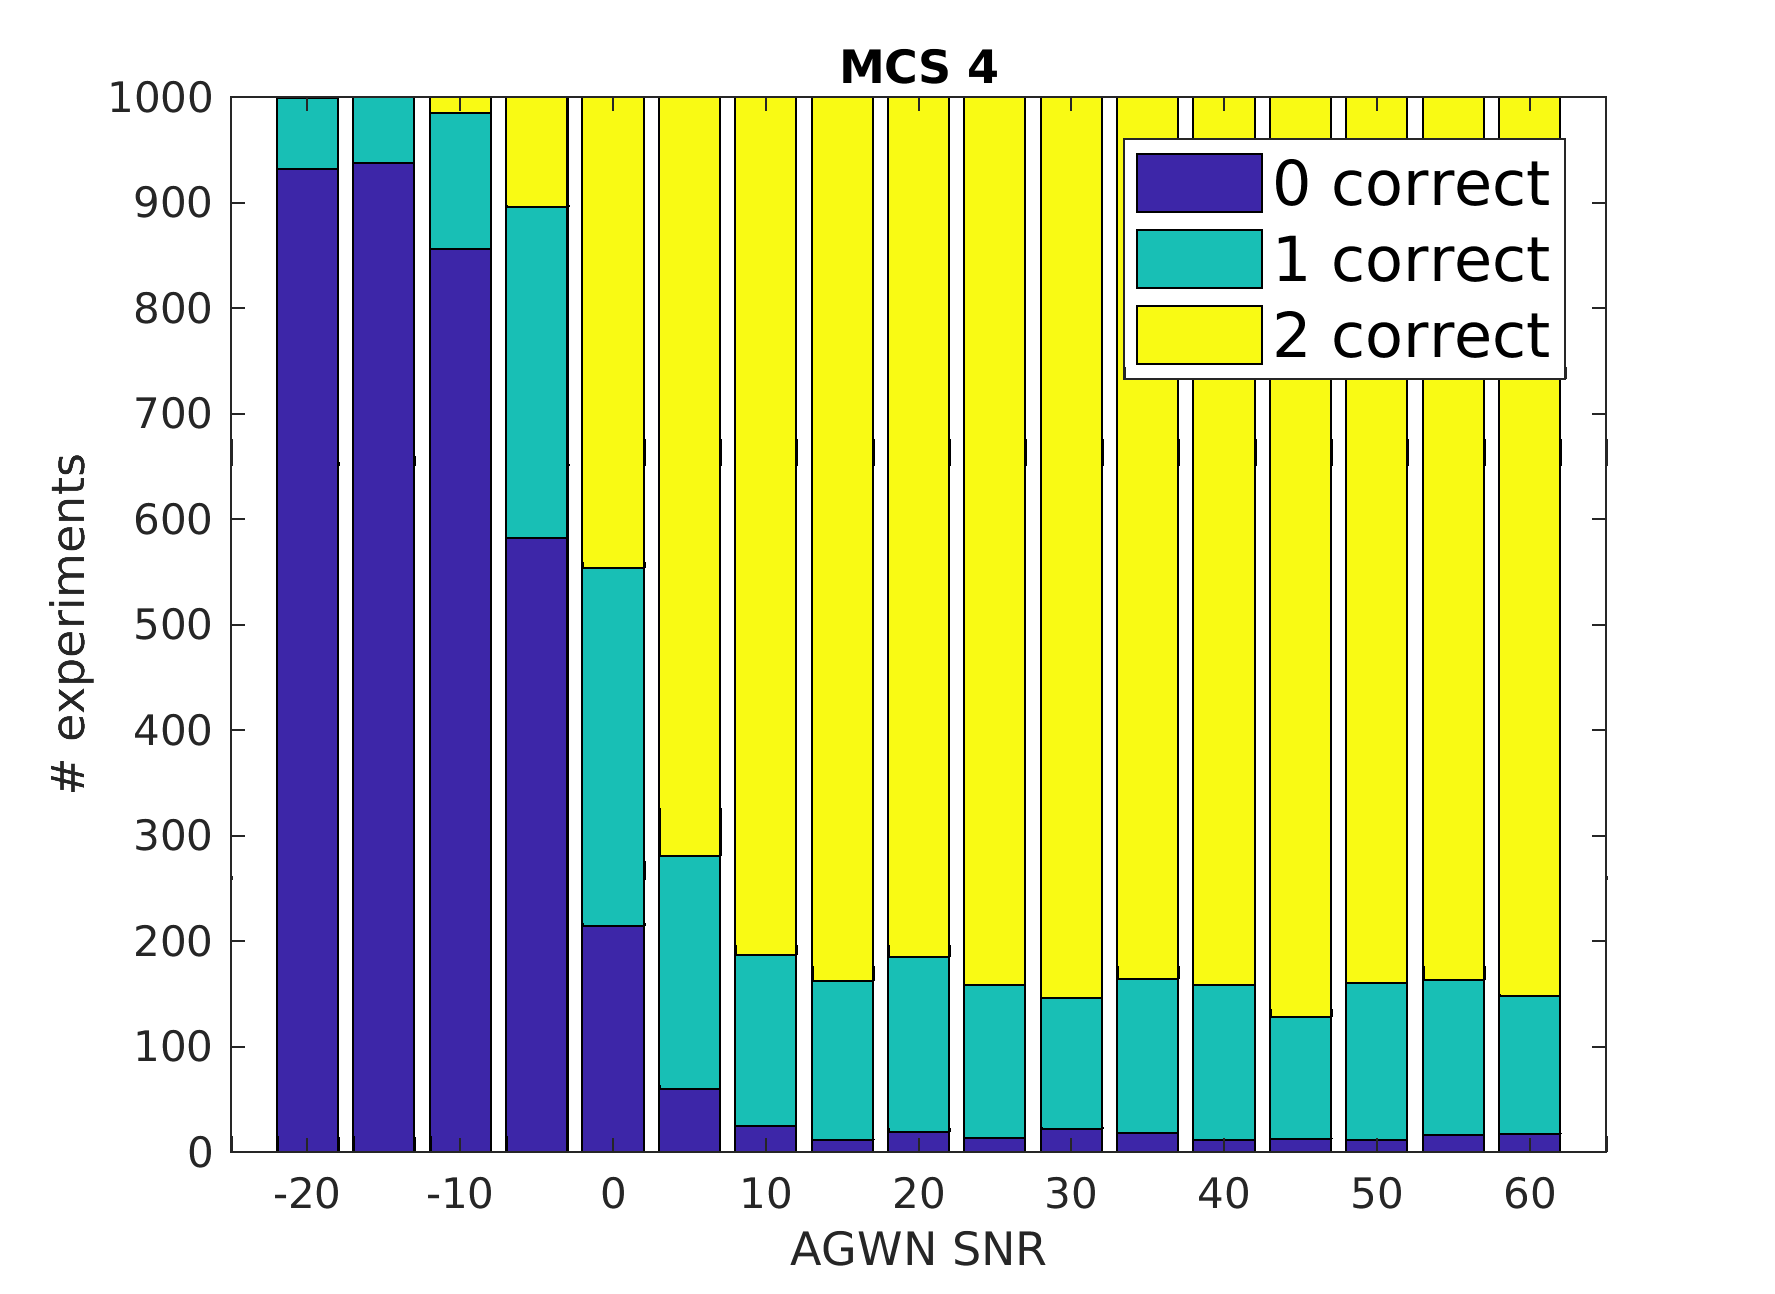
\includegraphics[width=0.42\textwidth]{gfx/plots/awgn-mcs4}} &
		\subfloat[MCS 5]{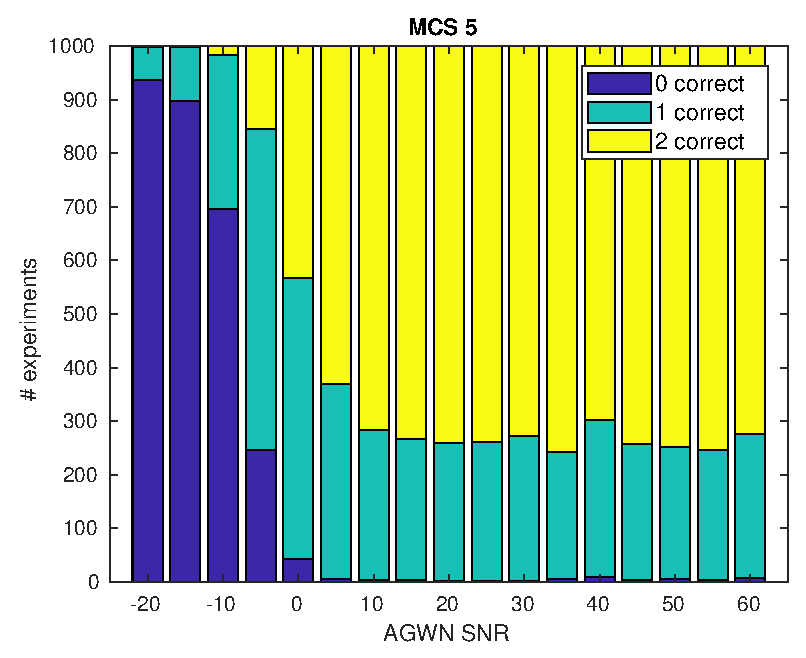
\includegraphics[width=0.42\textwidth]{gfx/plots/awgn-mcs5}} \\
		\subfloat[MCS 6]{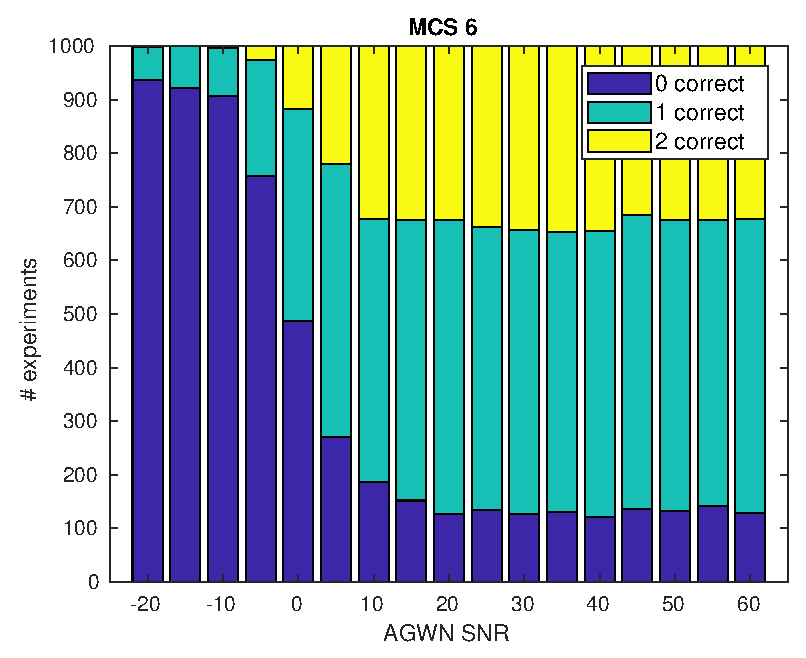
\includegraphics[width=0.42\textwidth]{gfx/plots/awgn-mcs6}} &
		\subfloat[MCS 7]{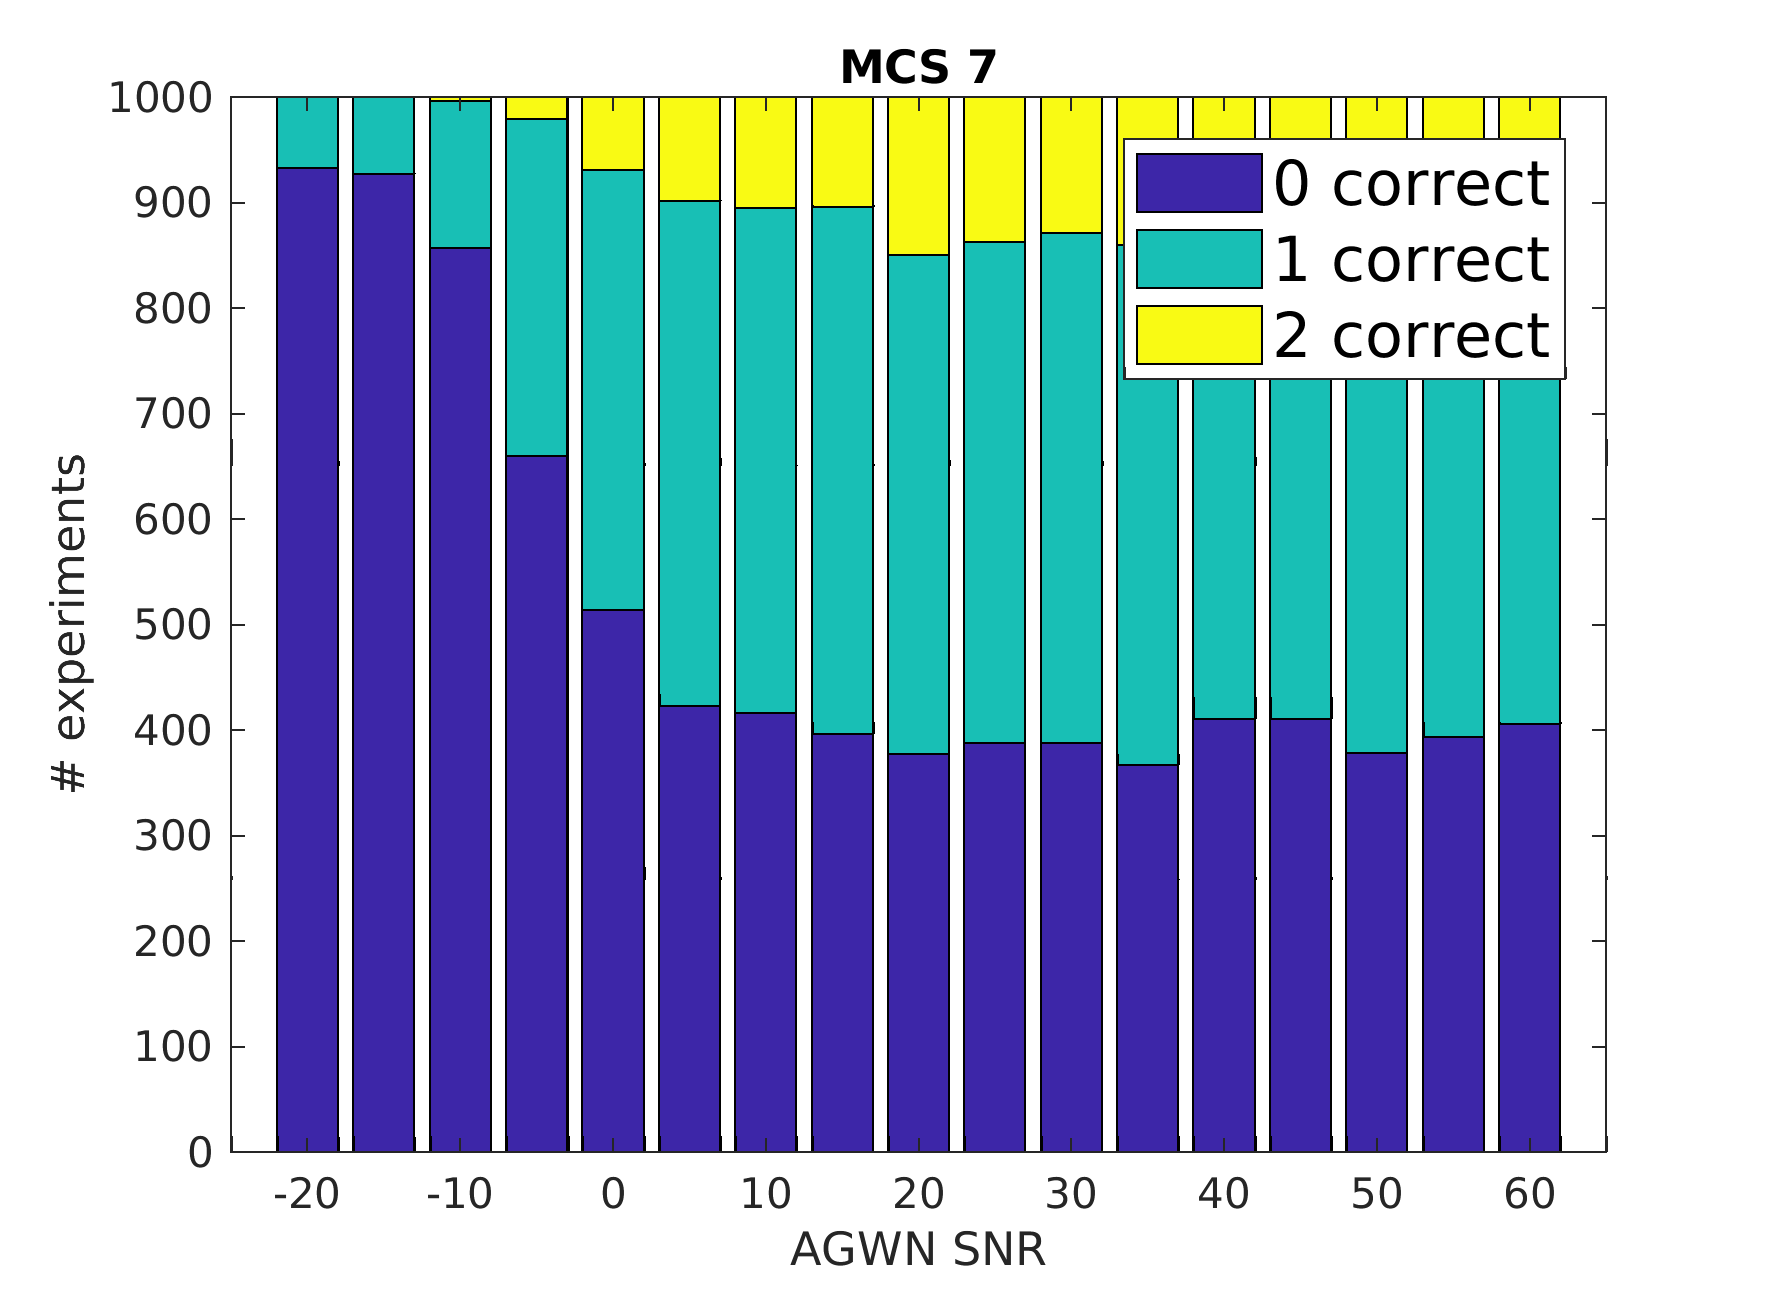
\includegraphics[width=0.42\textwidth]{gfx/plots/awgn-mcs7}} \\
	\end{tabular}
	\caption{Results: Varying AWGN SNR for 1000 Runs}
	\label{fig:vary_awgn}
\end{figure}

\begin{figure}[p]
	\centering
	\begin{tabular}{cc}
		\subfloat[MCS 0]{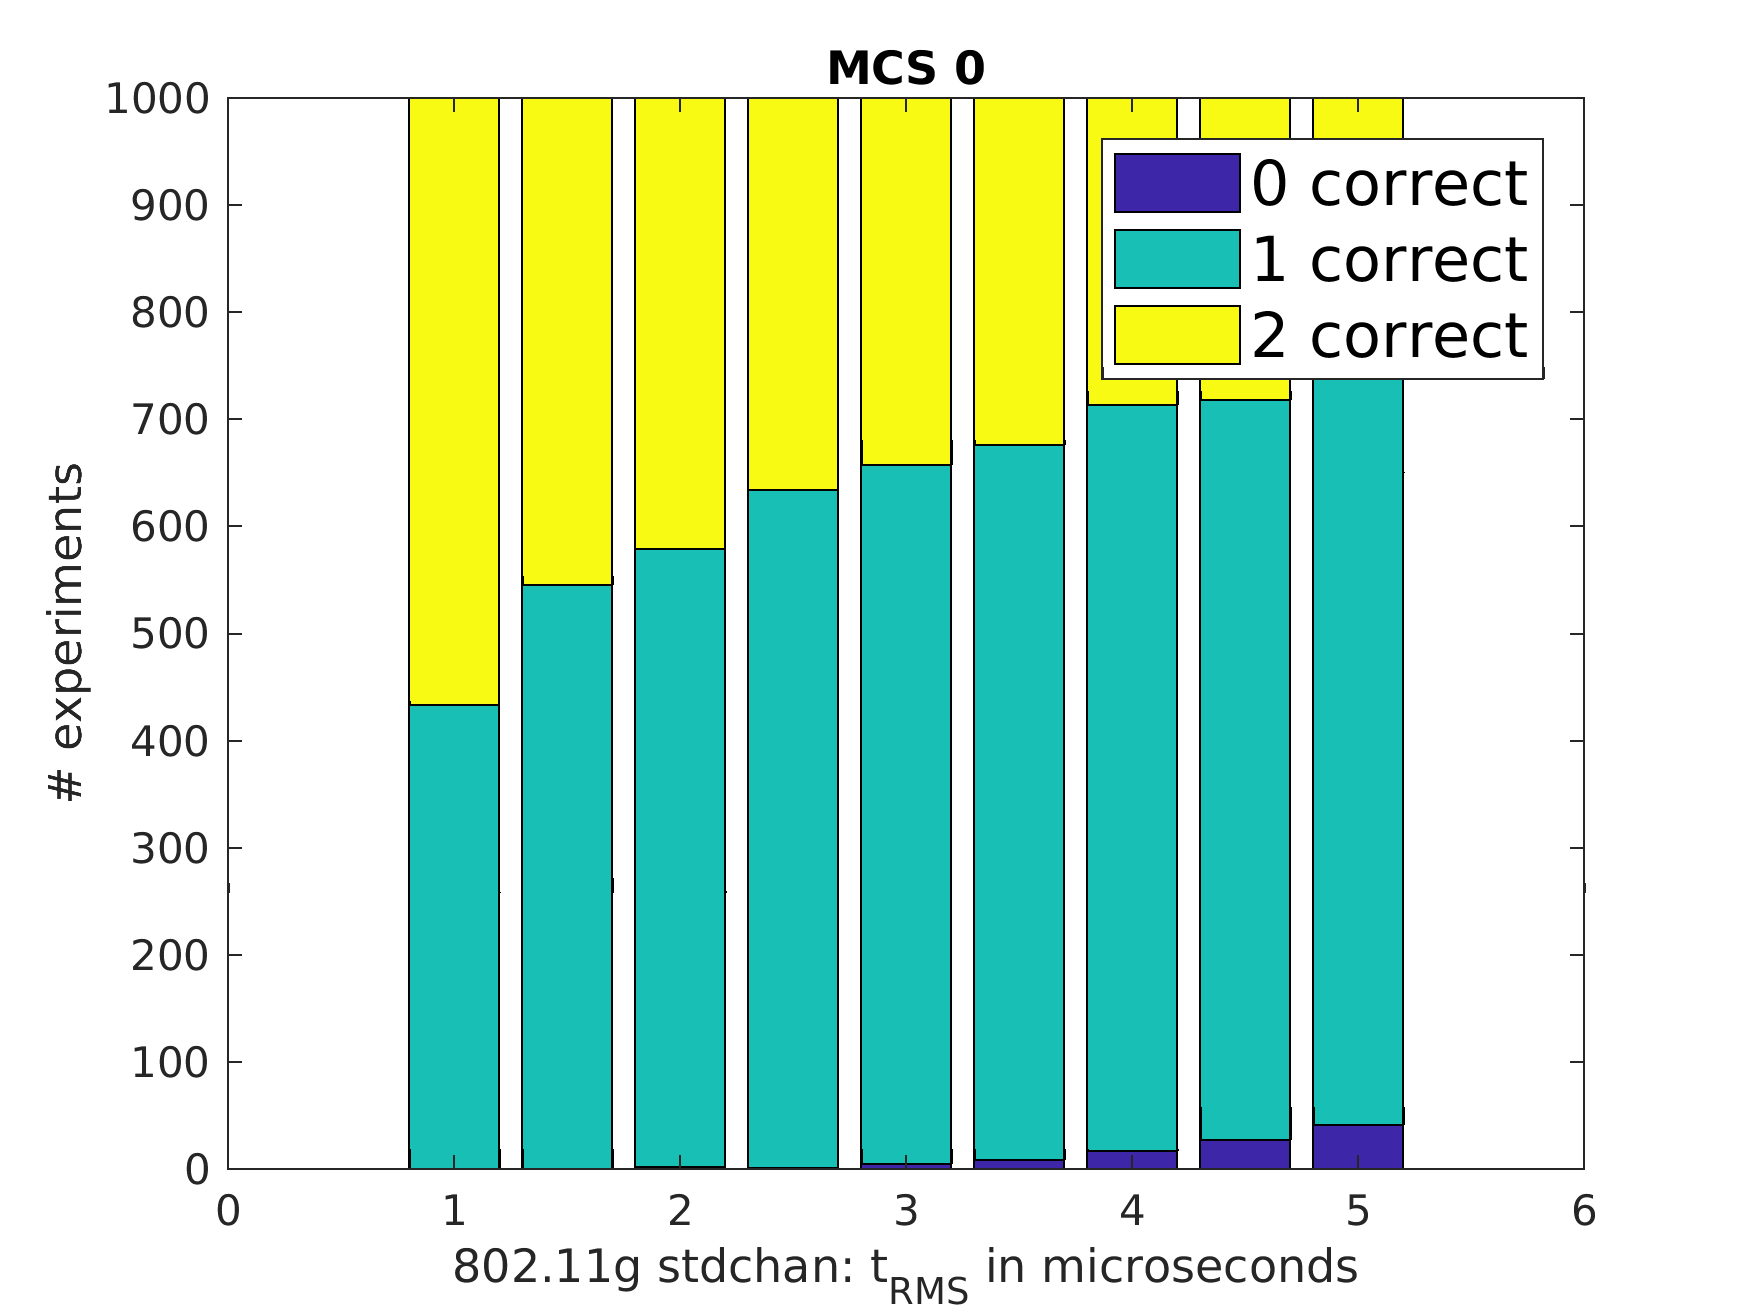
\includegraphics[width=0.43\textwidth]{gfx/plots/trms-mcs0}} &
		\subfloat[MCS 1]{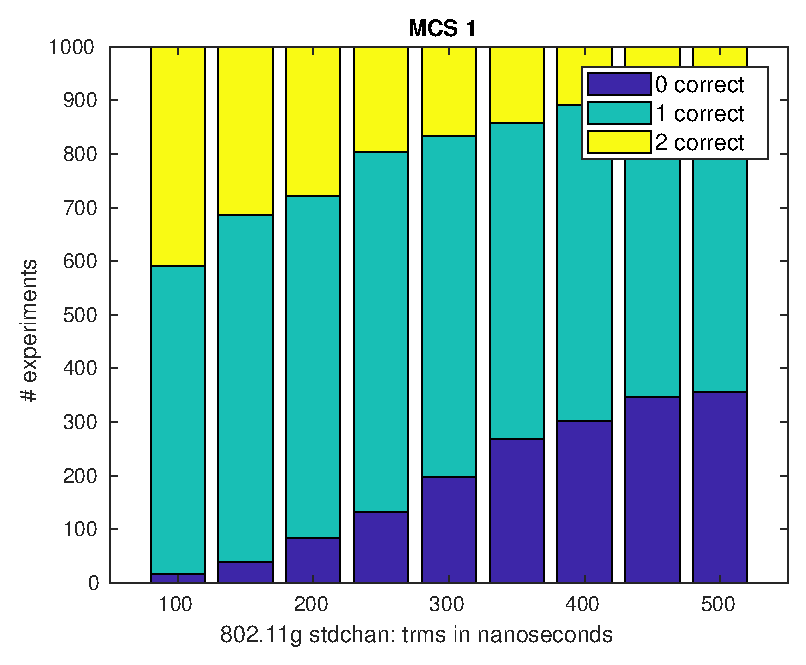
\includegraphics[width=0.43\textwidth]{gfx/plots/trms-mcs1}} \\
		\subfloat[MCS 2]{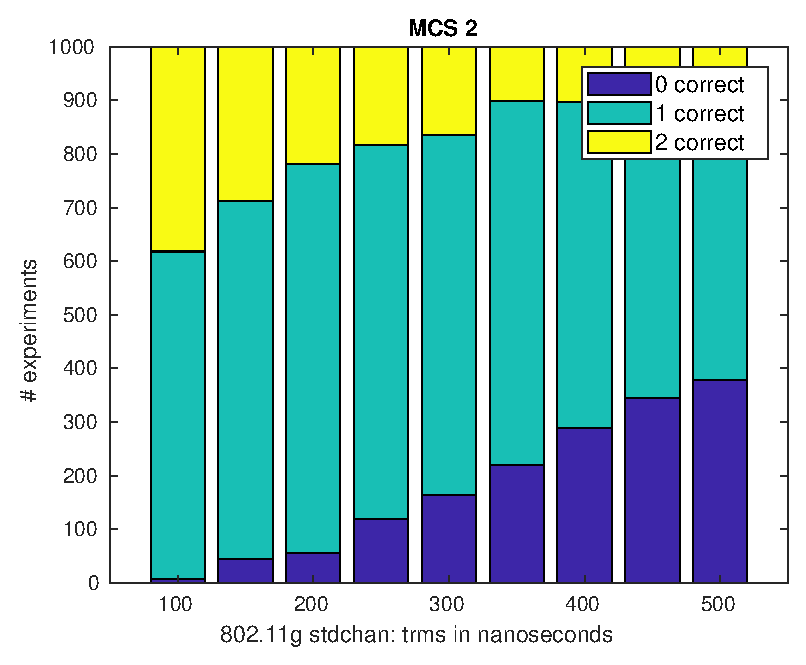
\includegraphics[width=0.43\textwidth]{gfx/plots/trms-mcs2}} &
		\subfloat[MCS 3]{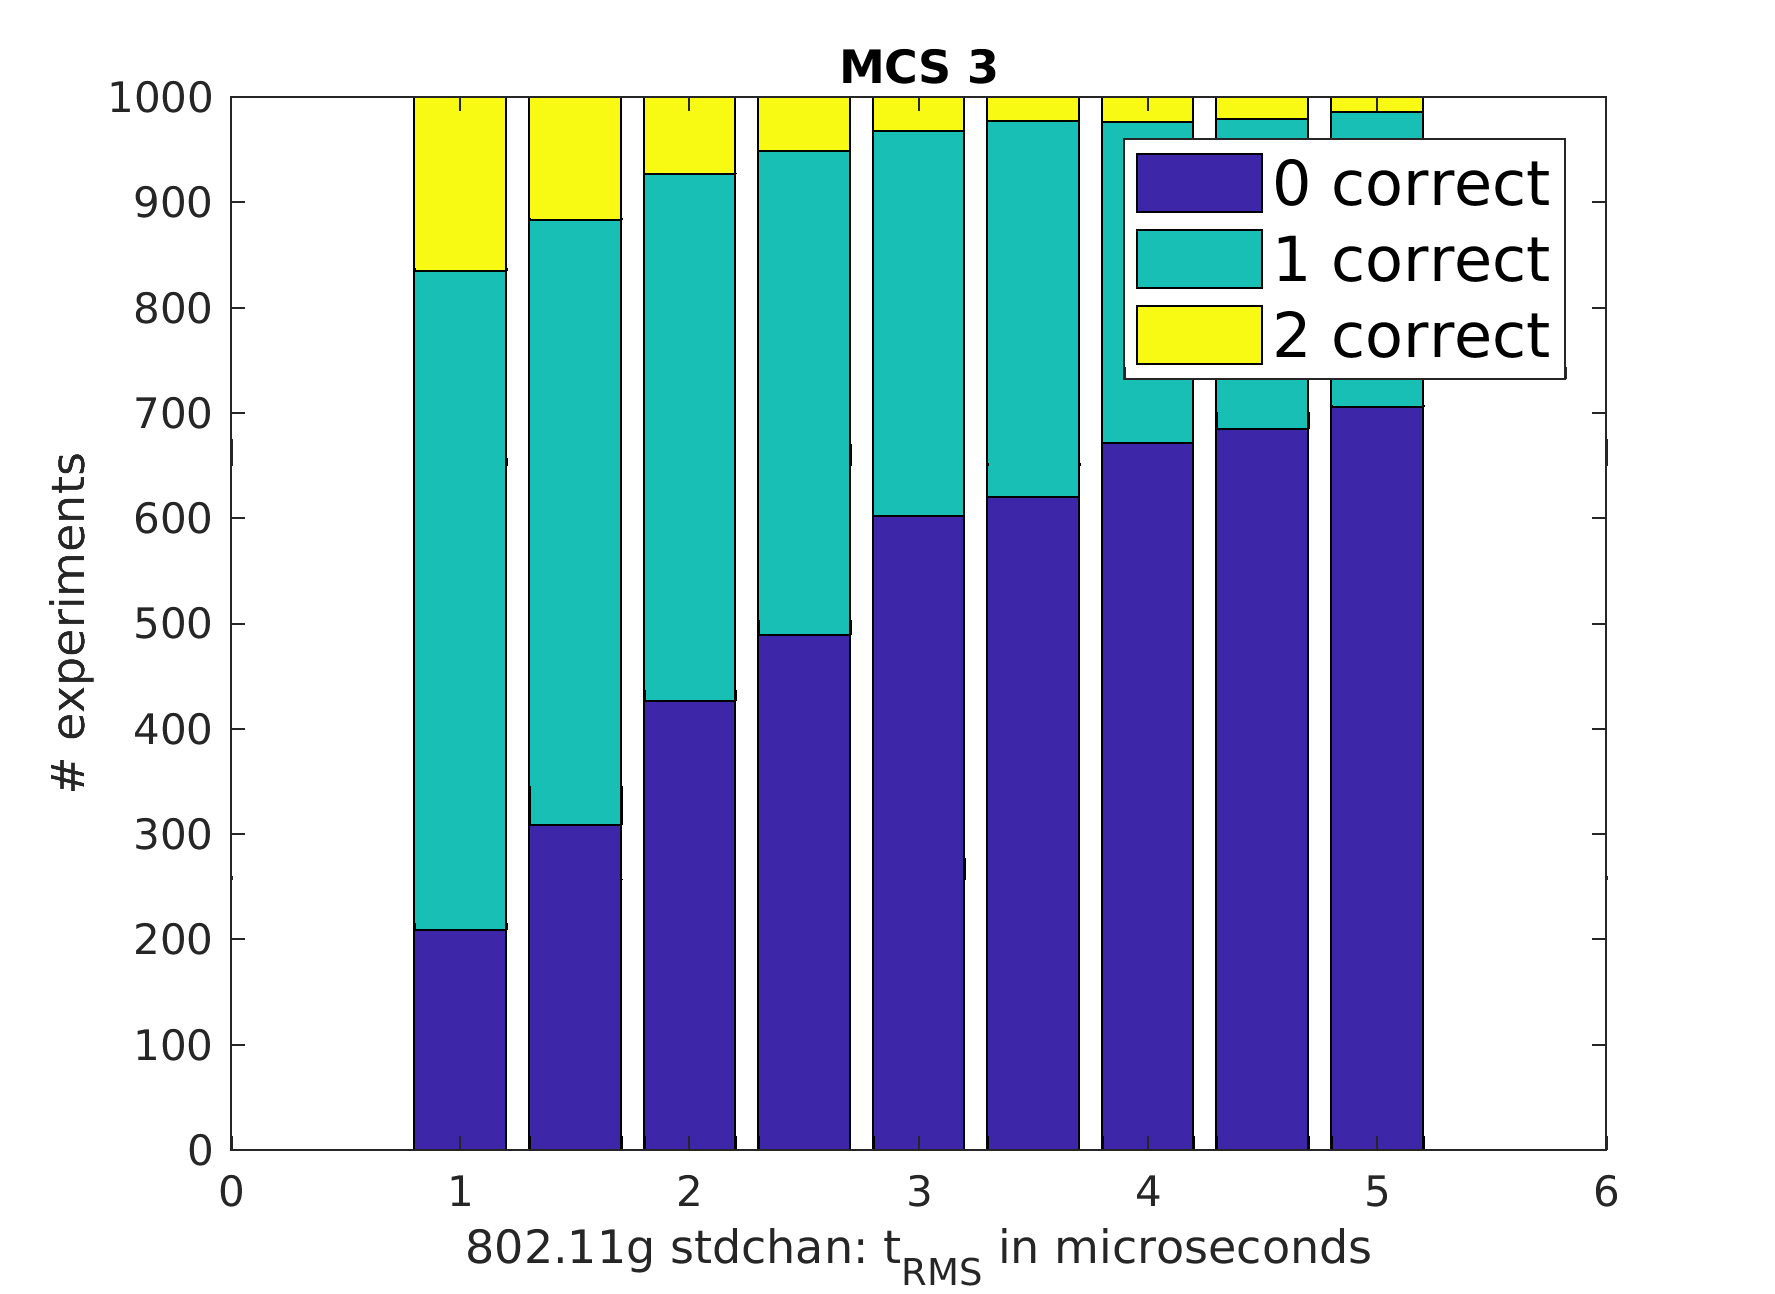
\includegraphics[width=0.43\textwidth]{gfx/plots/trms-mcs3}} \\
		\subfloat[MCS 4]{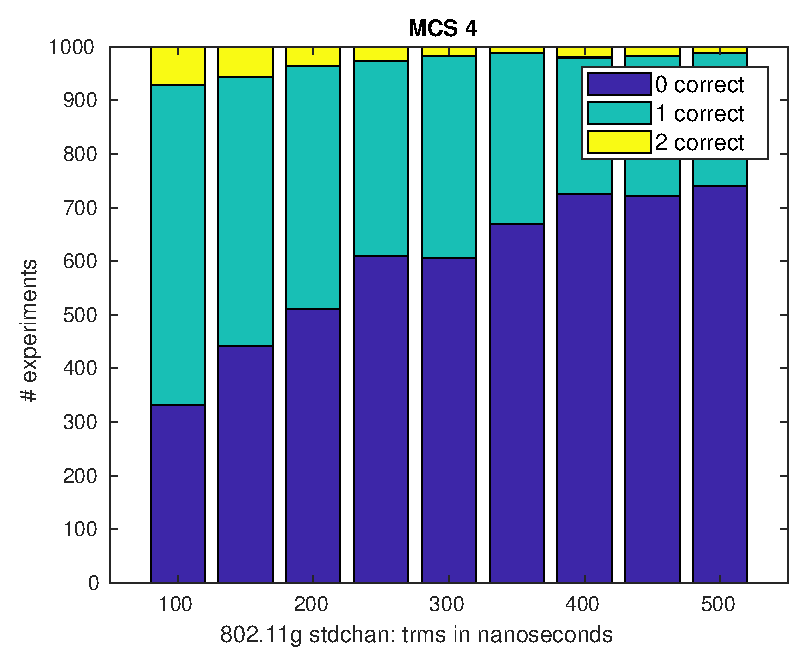
\includegraphics[width=0.43\textwidth]{gfx/plots/trms-mcs4}} &
		\subfloat[MCS 5]{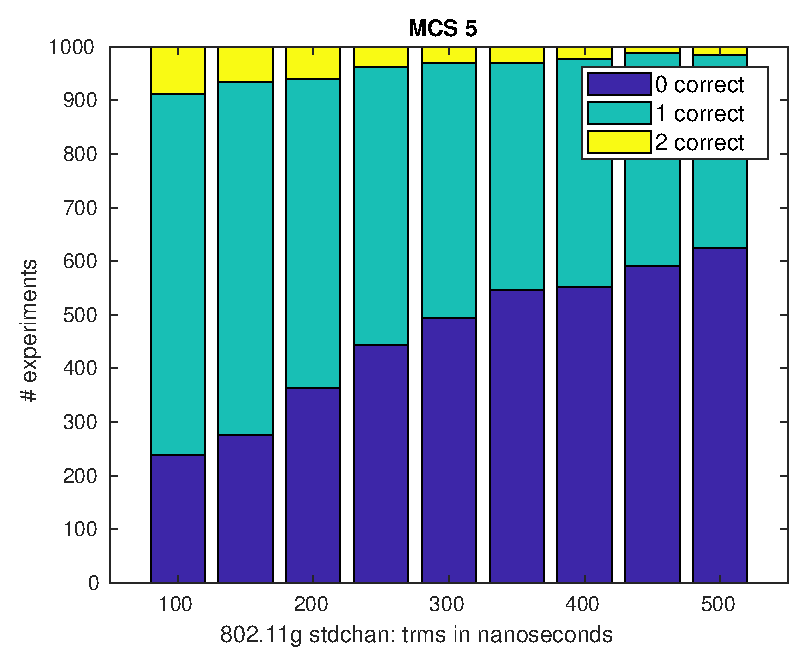
\includegraphics[width=0.43\textwidth]{gfx/plots/trms-mcs5}} \\
		\subfloat[MCS 6]{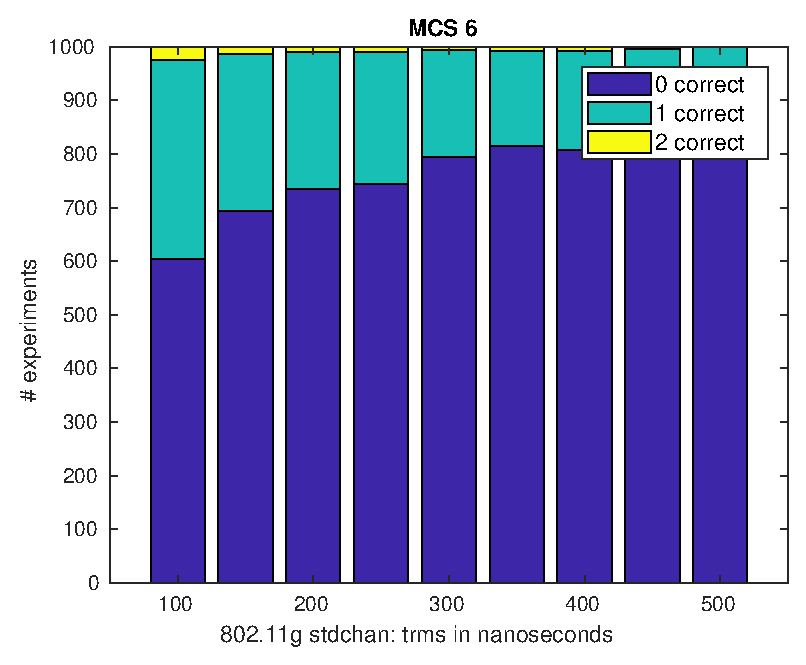
\includegraphics[width=0.43\textwidth]{gfx/plots/trms-mcs6}} &
		\subfloat[MCS 7]{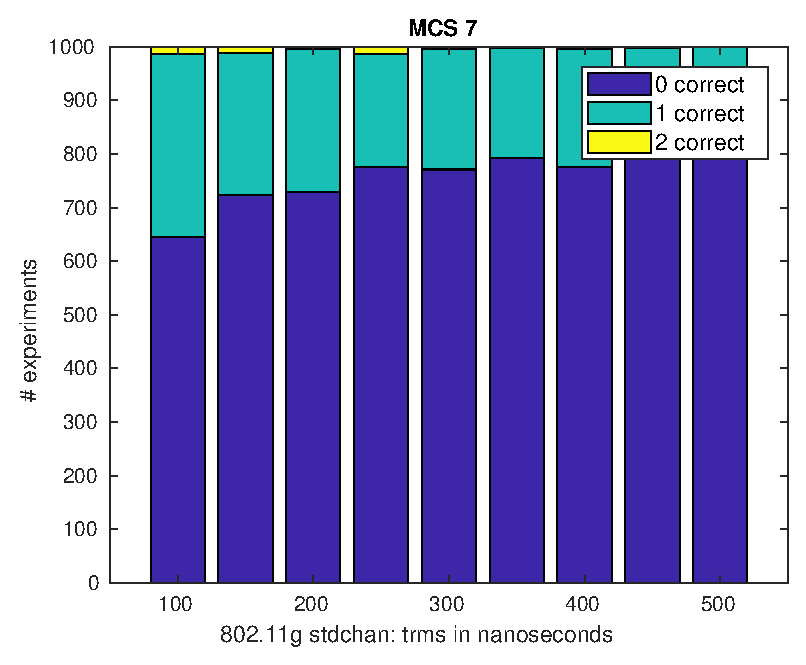
\includegraphics[width=0.43\textwidth]{gfx/plots/trms-mcs7}} \\
	\end{tabular}
	\caption{Results: Varying $t_{RMS}$ in a Standard Channel for 1000 Runs}
	\label{fig:vary_trms}
\end{figure}

\begin{figure}[p]
	\centering
	\begin{tabular}{cc}
		\subfloat[MCS 0]{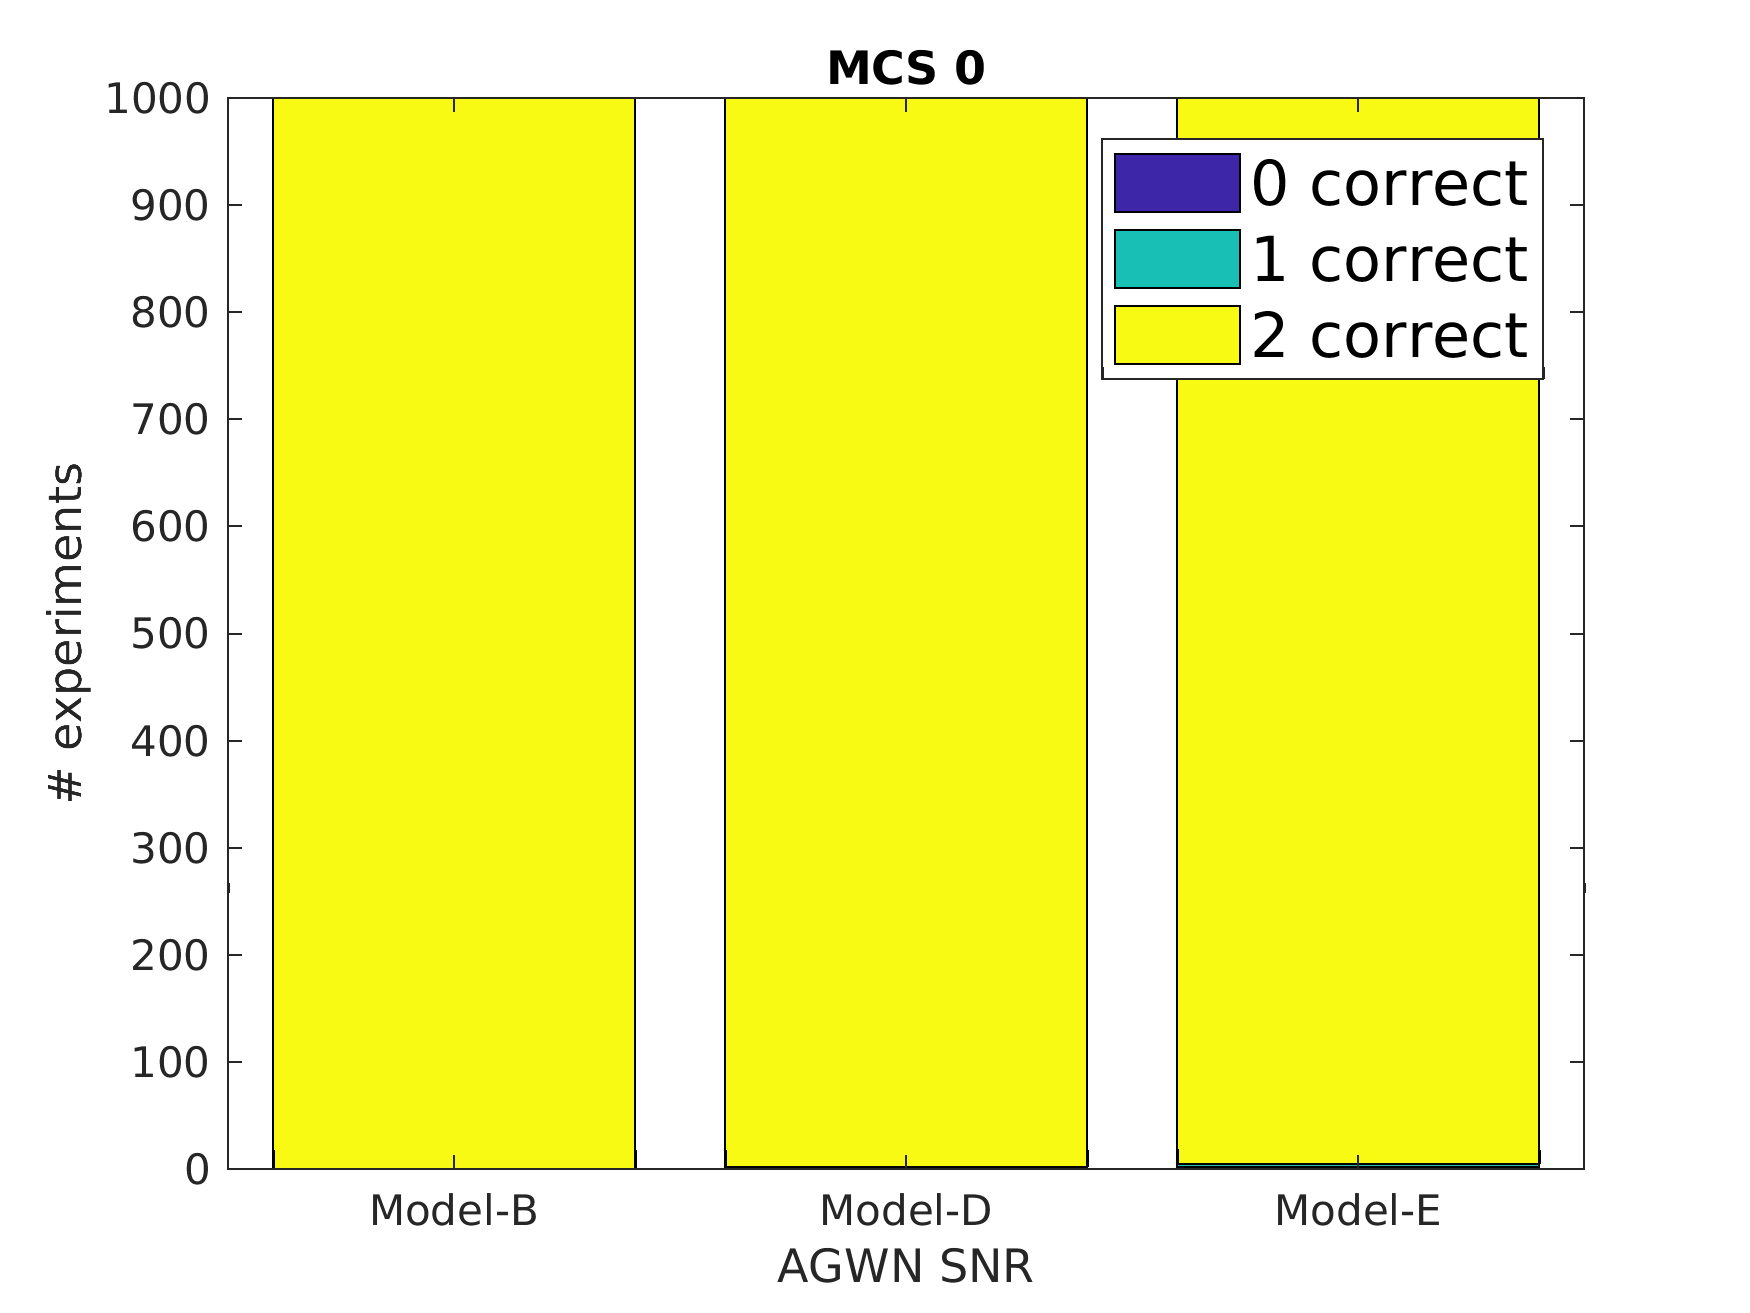
\includegraphics[width=0.42\textwidth]{gfx/plots/tgn-mcs0}} &
		\subfloat[MCS 1]{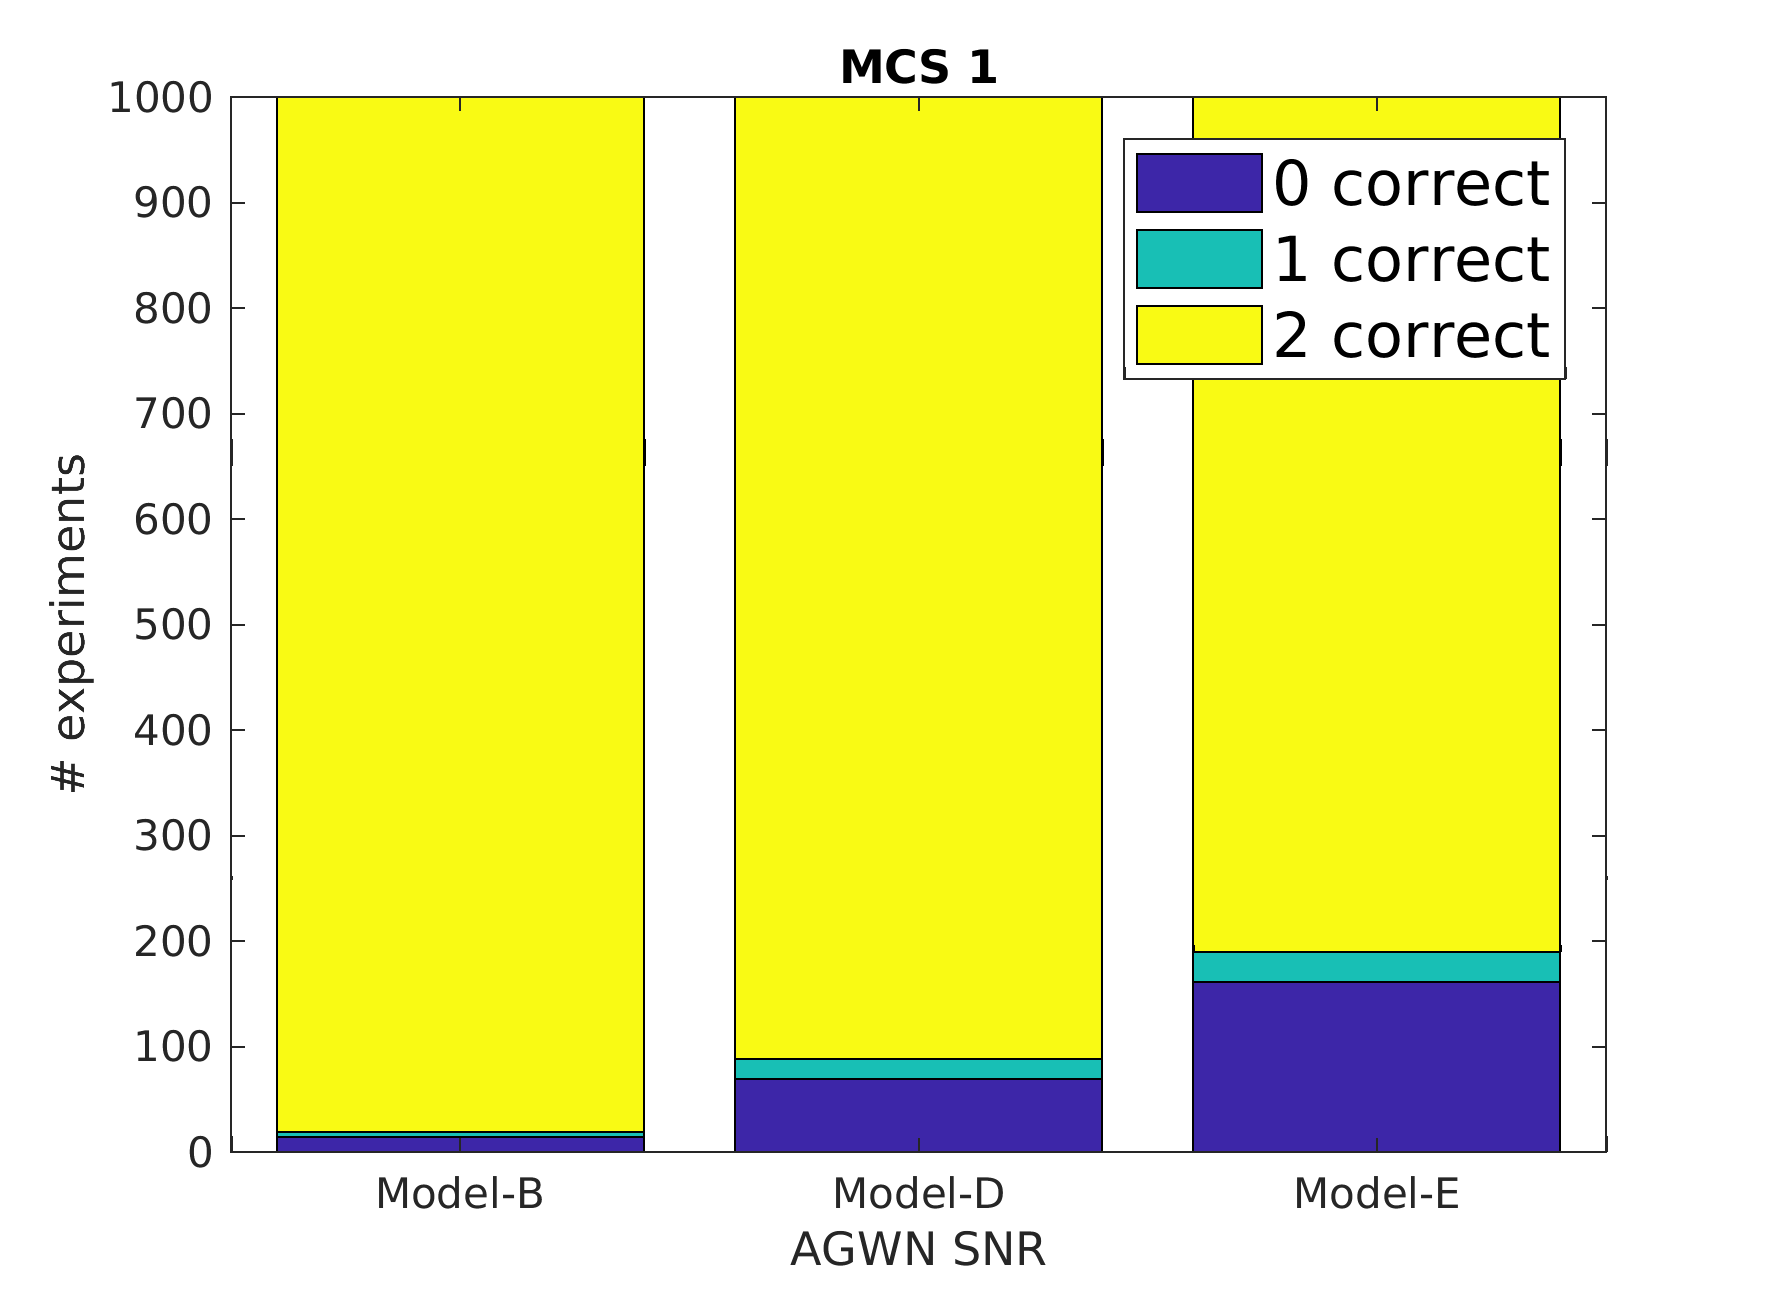
\includegraphics[width=0.42\textwidth]{gfx/plots/tgn-mcs1}} \\
		\subfloat[MCS 2]{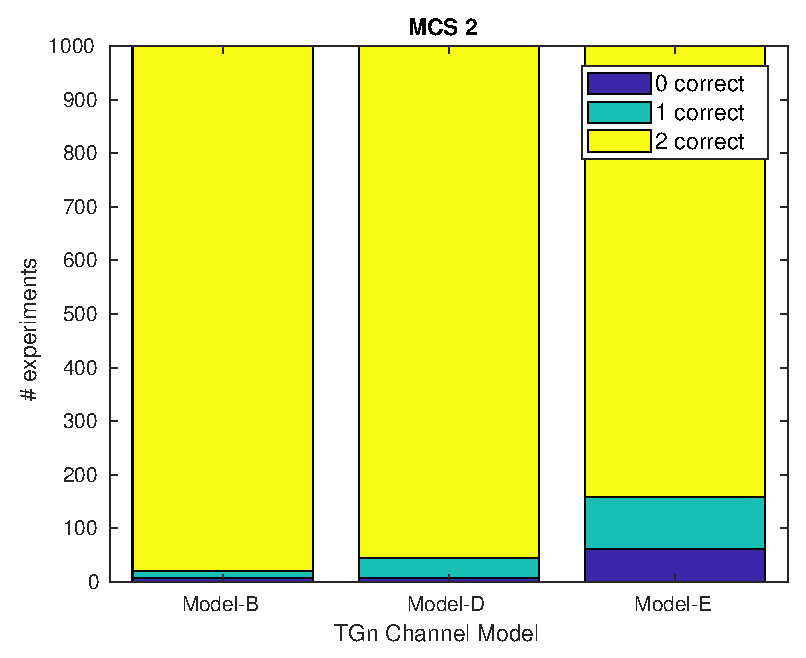
\includegraphics[width=0.42\textwidth]{gfx/plots/tgn-mcs2}} &
		\subfloat[MCS 3]{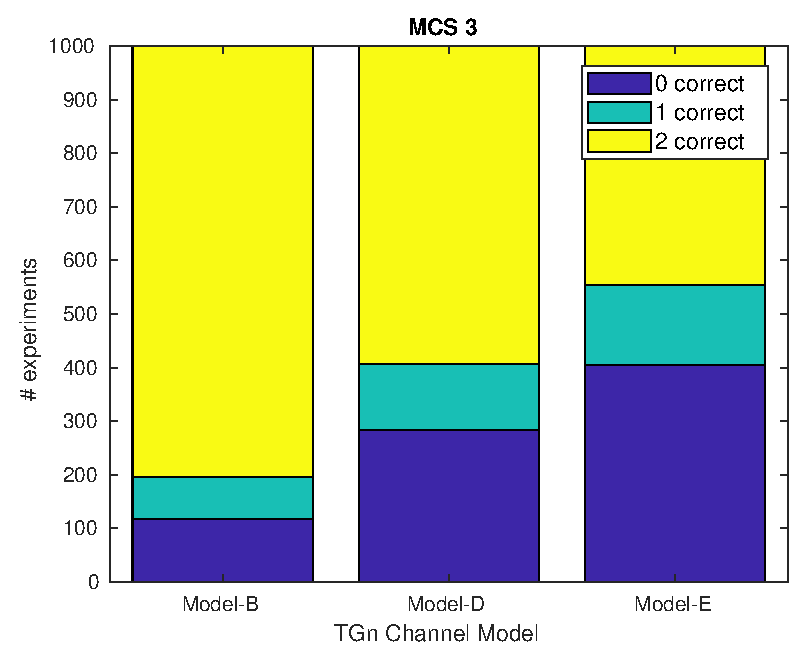
\includegraphics[width=0.42\textwidth]{gfx/plots/tgn-mcs3}} \\
		\subfloat[MCS 4]{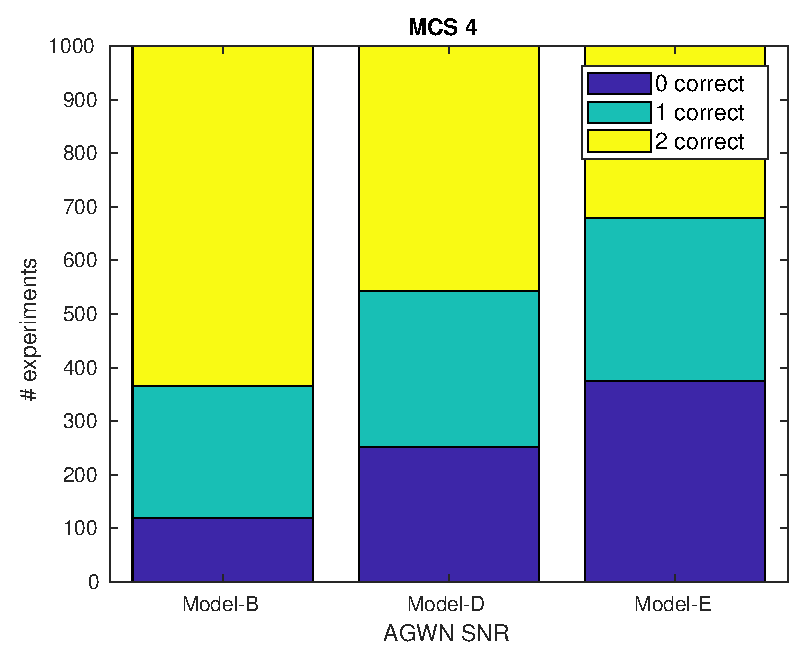
\includegraphics[width=0.42\textwidth]{gfx/plots/tgn-mcs4}} &
		\subfloat[MCS 5]{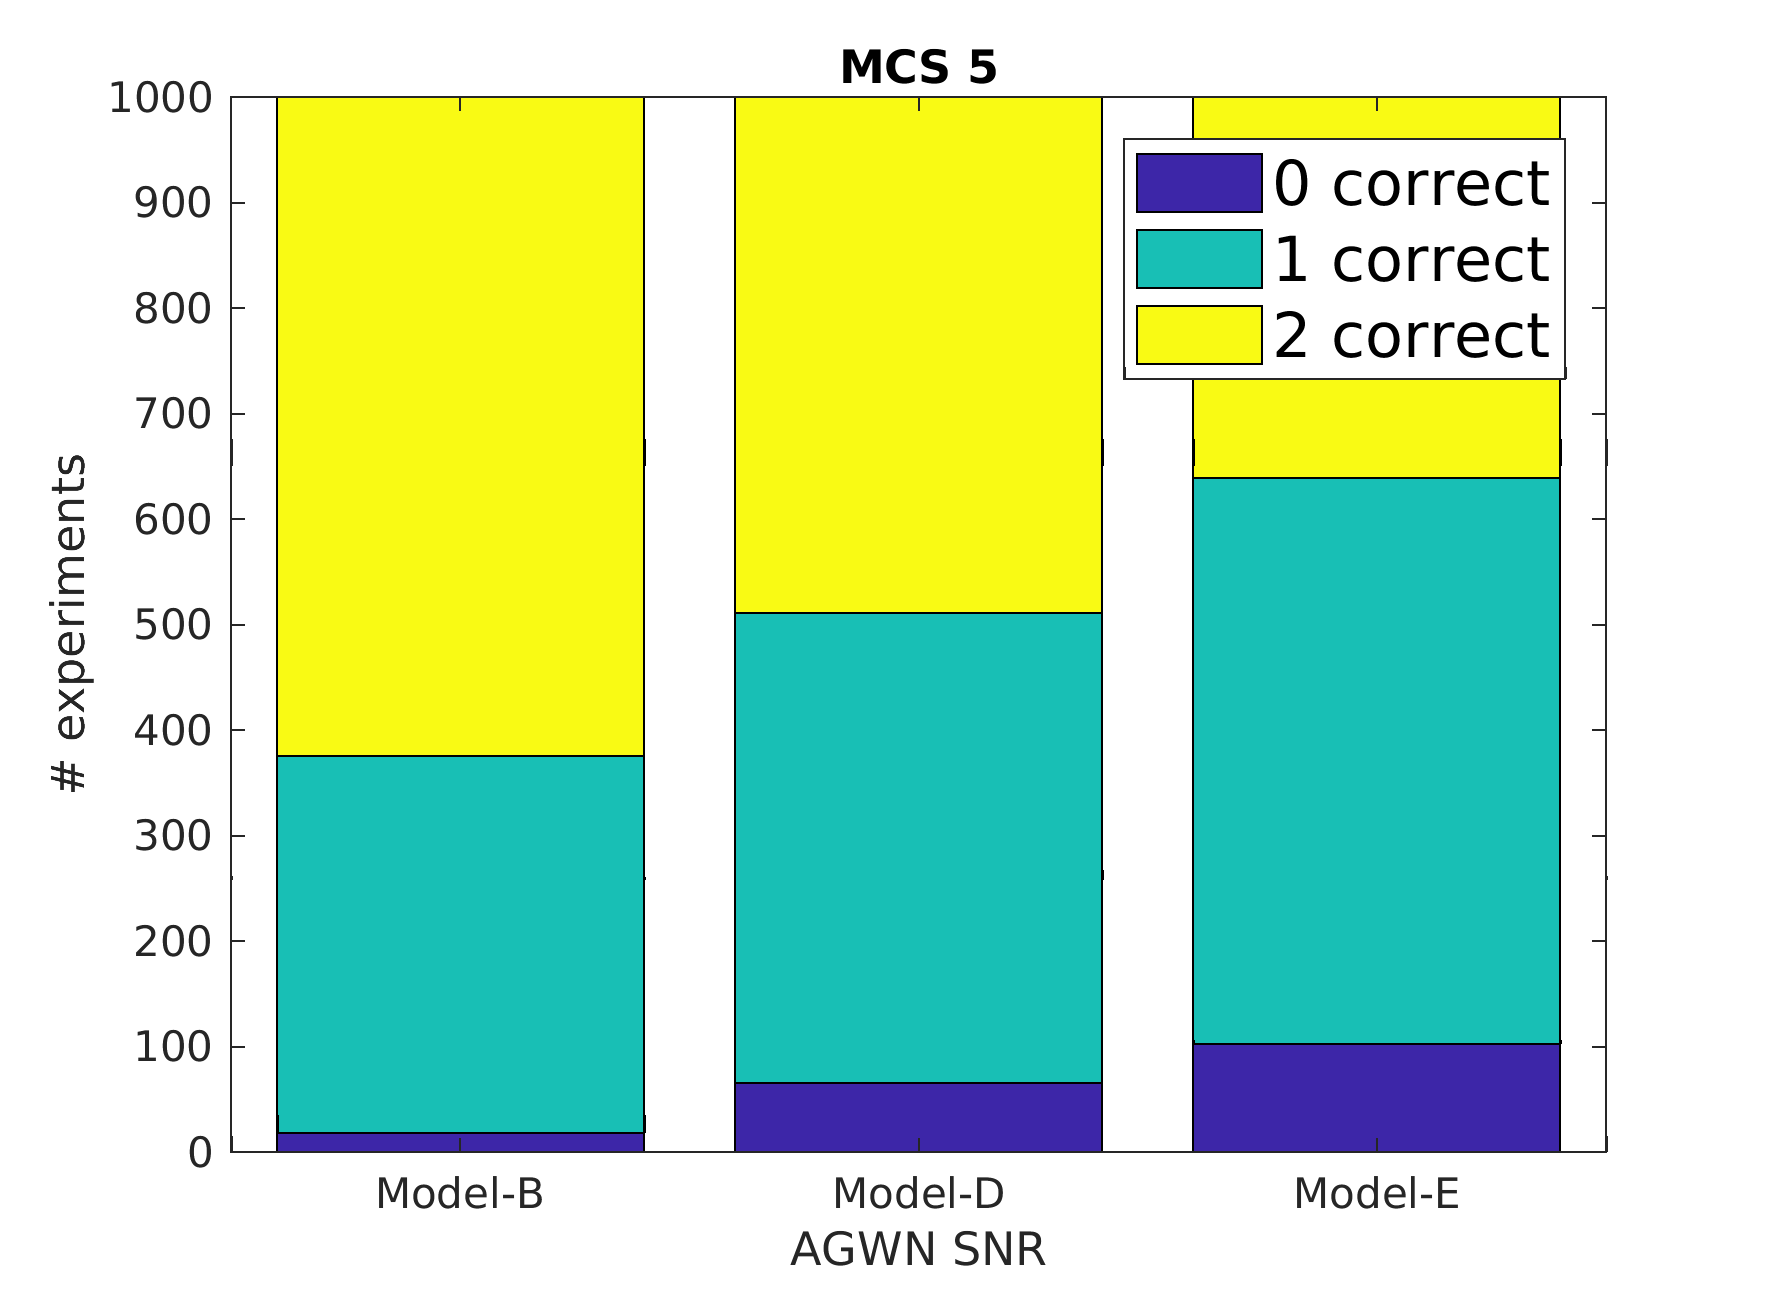
\includegraphics[width=0.42\textwidth]{gfx/plots/tgn-mcs5}} \\
		\subfloat[MCS 6]{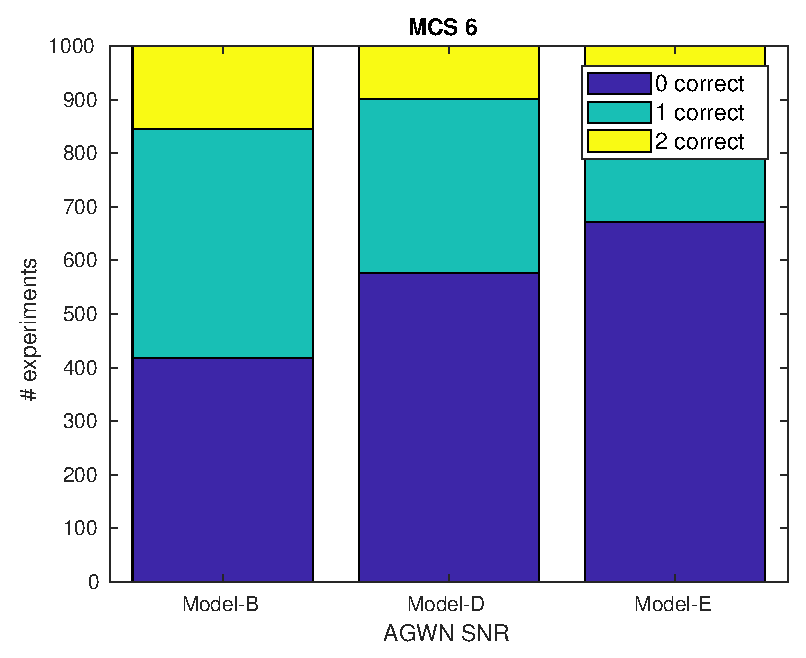
\includegraphics[width=0.42\textwidth]{gfx/plots/tgn-mcs6}} &
		\subfloat[MCS 7]{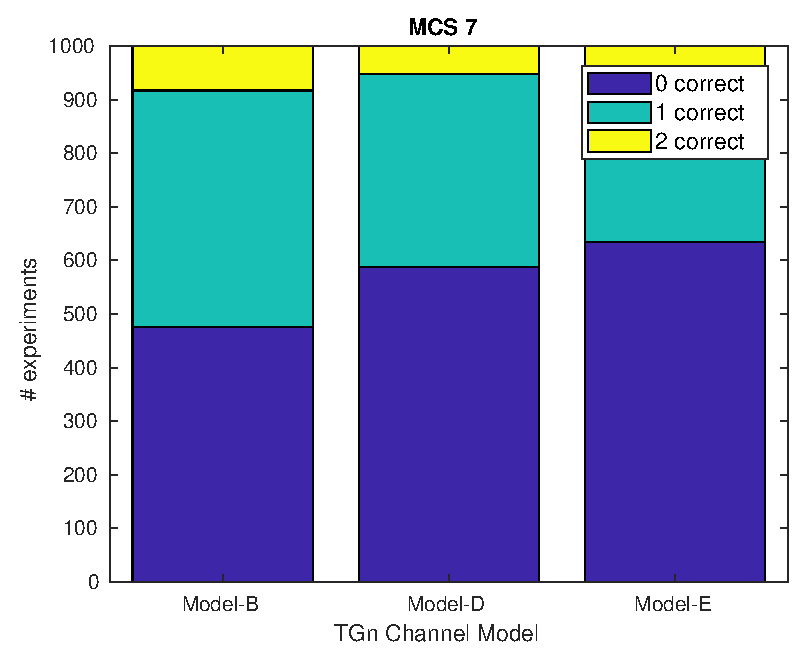
\includegraphics[width=0.42\textwidth]{gfx/plots/tgn-mcs7}} \\
	\end{tabular}
	\caption{Results: Varying TGn Channel for 1000 Runs}
	\label{fig:vary_tgn}
\end{figure}

%% -----------------------------------------------------------------------------

\section{WARP Experiments}\label{sec:ex-warp}

Lastly, I used \glspl{SDR} instead of pure software simulations to evaluate the sender detection performance with real-world channel effects. The experiments were conducted using three \gls{WARP} boards. I flashed all of them with the WARPLab reference design, version 7.5.1. Two \glspl{SDR} were used as senders, the remaining one acted as receiver. The \glspl{SDR} are connected to a controlling workstation using a gigabit Ethernet switch. The overall hardware layout is illustrated in figure \ref{fig:warp-layout}.

\begin{figure}[H]
	\centering
	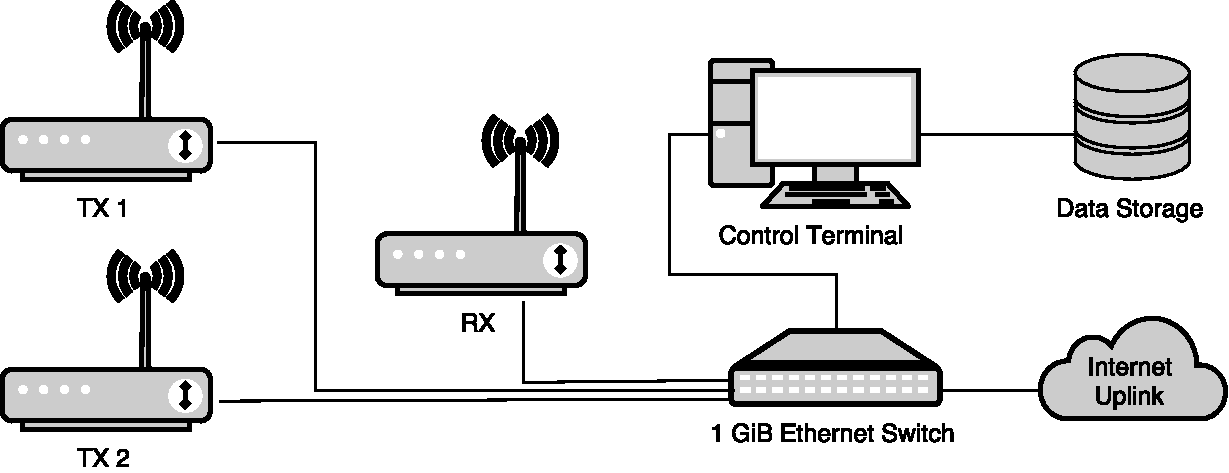
\includegraphics[width=\textwidth]{gfx/images/warp-layout}
	\caption{WARP SDR Experiments Hardware Layout}
	\label{fig:warp-layout}
\end{figure}

The experiments were carried out in a typical office building. This means that there were multiple IEEE 802.11 networks with several dozens of connected clients. I used a standard WLAN channel and no electromagnetic shielding.\\

Since the \gls{WARP} boards use a sampling frequency of 40 MHz, but the Matlab WLAN System Toolbox creates time-domain samples with a 20 MHz sampling rate, I used interpolation to adapt frequencies. This is done with the built-in \texttt{resample} Matlab function. Listing \ref{lst:resample} illustrates the process.

\begin{lstlisting}[captionpos=b,caption={Interpolate Sampling Rate},label=lst:resample]
% Interpolate to get from 20 to 40 MHz sampling rate
tx1 = resample(tx1, 40, 20);
\end{lstlisting}

For the real-world experiments, I deliberately caused frame collisions with the same scrambler initialization and destination \gls{MAC} addresses, and used \gls{MCS} 0. This means that in principal everything was the same as for the most basic simulation experiments.

To assess the basic mechanics of receiving collisions with the \glspl{SDR}, I applied cross-correlation to only one \gls{LTF} symbol instead of the \gls{MAC} addresses and plotted the results. They are presented in figure \ref{fig:warp_preamble_corr}. The collided frames were aligned with some offset for this experiment.

While one group of spikes is slightly lower than the other, it is still easily possible to detect that there is a collision due to the four higher and two lower spikes caused by the two \glspl{LTF}. The higher level of noise in the beginning of the signal are probably caused by \gls{AGC} in the receiving \gls{SDR}. Since the \gls{MAC} addresses are located further into the signal, and only that part is correlated for sender detection, this noise should be no problem.

\begin{figure}[H]
	\centering
  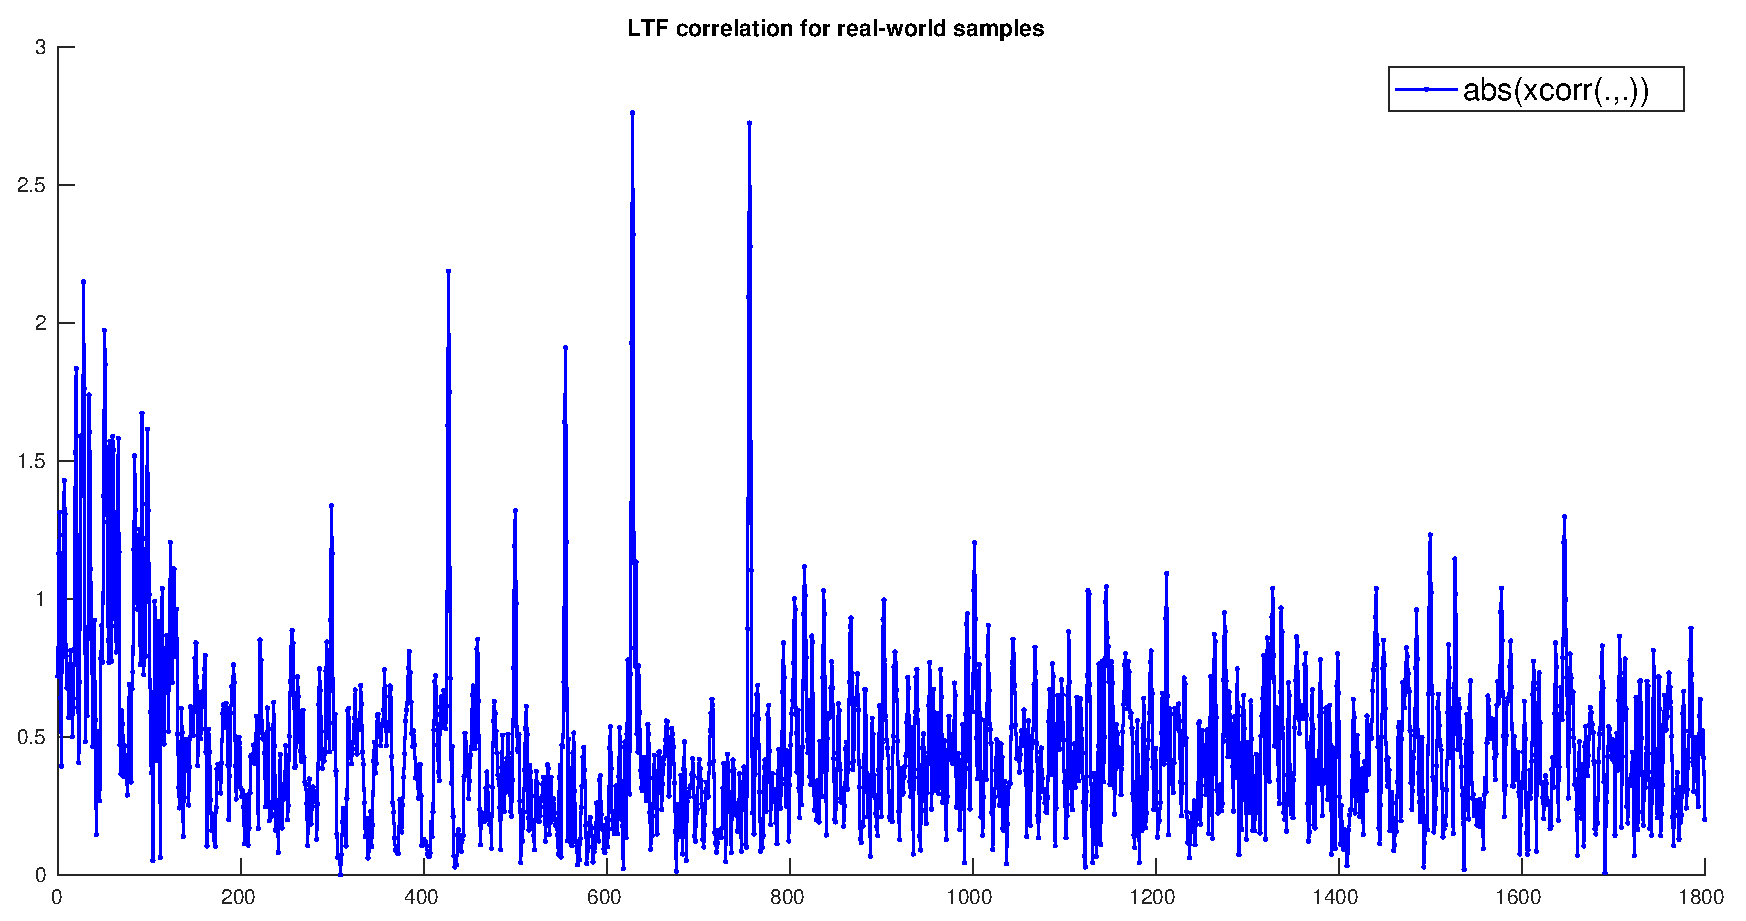
\includegraphics[height=5.5cm]{gfx/plots/warp-preamble}
	\caption{Preamble Correlation on WARP SDRs}
	\label{fig:warp_preamble_corr}
\end{figure}

The results of the preamble correlation are promising. They show that indeed a collision of two frames is captured by the receiving \gls{SDR}, and that cross-correlation in the time-domain can in fact distinguish both \glspl{LTF}.\\

Next, I used the same code as for the simulation experiments to try and detect sender \gls{MAC} addresses. This worked reasonably well despite some problems. The results are shown in figure \ref{fig:warp-mcs-results}. I used \glspl{MCS} 0 to 5 with a total of 10 runs each.

\begin{figure}[H]
	\centering
	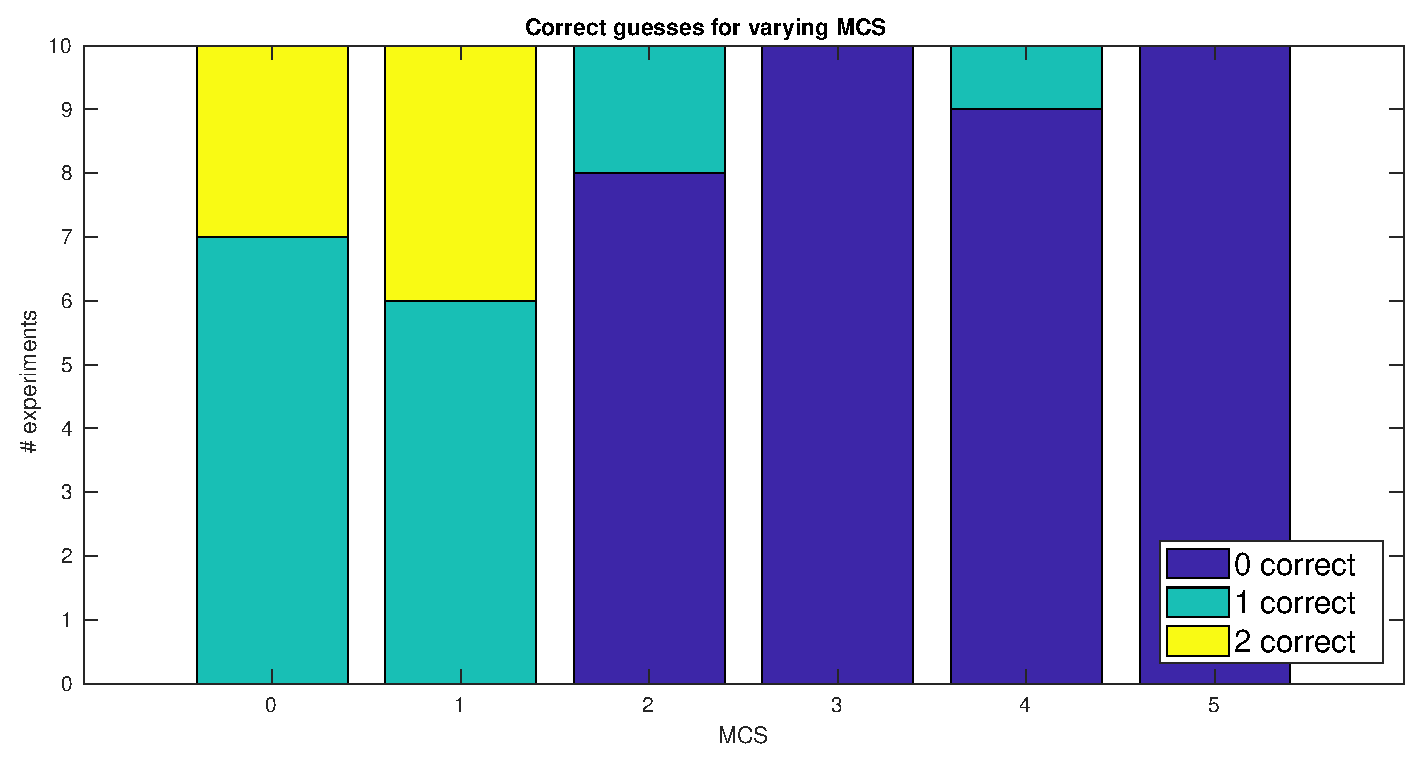
\includegraphics[height=4.5cm]{gfx/plots/warp-mcs}
	\caption{Results: Varying MCS for 10 Runs on WARP SDRs}
	\label{fig:warp-mcs-results}
\end{figure}

For \glspl{MCS} 0 and 1, the results were quite good. Although in most of the cases only one \gls{MAC} address could be detected correctly, investigations showed that the correctly guessed address was transmitted by the same \gls{SDR} every time. This hints that there could be some environmental factors causing its signal to be received more strongly. Another thing is that wrong guesses were often due to quite similar \gls{MAC} addresses, which were different in only a few bits.

However, for higher \glspl{MCS}, sender detection seemed to fail. This is probably caused by real-world channel effects, that could not be simulated to a realistic extent.
